\documentclass{article}
\usepackage[utf8]{inputenc}
\usepackage{amsmath}
\usepackage{graphicx}
\usepackage{geometry}

\geometry{
	a4paper,
}

\begin{document}
\Large
\tableofcontents
\newpage
\section{Introduzione}
Terminologia:
\begin{itemize}
\item Sistema: insieme di risorse hardware e software
\item Metriche: criteri per confrontare le prestazioni del sistema, qualsiasi esso sia. Ad esempio:
\begin{itemize}
\item il tempo di risposta
\item throughput: "produttività" del sistema per unità di tempo, in base a cosa il sistema produce (es richieste per unità di tempo)
\end{itemize}
\item Workload: richieste che gli utenti sottomettono per un servizio che il sistema fornisce. Esempi:
\begin{itemize}
\item istruzioni CPU che un certo server può ricevere
\item query al DB
\end{itemize}
\item Tecnica: misure, simulazioni e modelli analitici
\end{itemize}
\subsection{Importanza del perfomance modelling}
Nonostante viviamo e sperimentiamo la sua importanza quotidianamente, ha una sensibilità poco importante. Ultimi anni:
\begin{enumerate}
\item Google down: 14/12/2020, problema per cui per circa 2h e 15 min tutti i servizi sono andati giù su scala mondiale. Didattica a distanza e smart working bloccati.\\ Problema è stato il blocco di qualsiasi servizio per l'accesso tramite autenticazione e quindi tutte le applicazioni coinvolte. La capacità ridotta del sistema centrale di gestione delle identità e di autenticazione di Google
\item Cashbak IO Pagopa: 7-10/12/2020. Milioni di donwload e di accessi, fino a 14000/s ed un autenticazione molto lenta, le troppe richieste hanno saturato le porte disponibili per l'accodamento delle richieste.\\ Blocco nell'inserimento dei metodi di pagamento, con annesso crollo dei servizi di push (che mette in coda le richieste che arrivano), dovuto alla lentezza dell'autenticazione.\\ Bottleneck nell'autenticazione e problema nella gestione non appropriata delle richieste
\item Signal: 16/01/2021, aumento improvviso dei download del circa 4200\% in una settimana. Primo rallentamento del servizio, seguito da una parziale interruzione. La soluzione è stata di creare una replica del back-end su altri server.
\end{enumerate}
Moltissimi altri casi di questo tipo, oggi i sistemi hanno un livello di complessità molto alta come anche la loro composizione che è più complessa, la loro evoluzione è sempre più rapida. Inoltre, sono sempre più essenziali per il business e questo richiede la necessità di strumenti e tecniche che assistano progettisti, service provider etc... che permettano di capire a pieno il comportamento dei sistemi, in tutte le fasi:
\begin{itemize}
\item Progetto ed implementazione
\item Dimensionamento
\item Vita ed evoluzione del sistema 
\end{itemize}
Tutte le tecniche per la valutazione delle prestazioni consentono anche una visione ed una conoscenza del sistema che il sistema stesso non offre: studiare il comportamento mediante un modello consente di vedere aspetti che non avremo potuto vedere in altro modo.\\ Tutte le figure che hanno a che fare con sistemi di questo tipo devono avere un background di tecniche di valutazione delle prestazioni.
\subsection{Valutazione delle performance}
Non è importante solo a livello industriale, ma anche nella ricerca accademica, nel momento in cui si vuole valutare una nuova proposta. Anche in questo caso la modellazione può essere molto utile. Nell'industria è essenziale per mantenere dei livelli di qualità alti, espressi negli SLA: il service provider deve poter identificare in maniera rapida dove c'è un problema che potrebbe portare al crollo delle performance garantite (per non andare in contro a penali) e di fare un tuning del sistema per ritornare al livello di qualità che doveva essere garantito.\\ Un buon modello di valutazione delle prestazioni ci da una conoscenza profonda del comportamento del sistema: perché il sistema si comporta in un certo modo e perché lo fa, quali sono i limiti di quel comportamento ed i punti critici nel caso ci fossero problemi e fosse necessario migliorare le performance.
\subsubsection{Obiettivi della valutazione delle performance}
Alcuni esempi e obiettivi per un sistema:
\begin{itemize}
\item Capicity planning: determinare il numero e la taglia dei componenti del sistema
\item Tuining del sistema: messa a punto del sistema, quando c'è qualcosa che si evidenzia nel comportamento del sistema che porta al degrado delle performance, bisogna determinare l'ottimo per il valore del parametro
\item Bottleneck identification: determinare le performance di un bottleneck, identificarlo per poter capire qual'è la risorsa che saturerà per prima.
\item Caratterizzazione del carico: solitamente ben modellate con distribuzioni esponenziali (o al più a fase), quindi che hanno la maggior parte della loro probabilità distribuite su valori piccoli, ovvero con tempi piccoli. Le probabilità di valori grandi sono piuttosto basse. Heavy-tail, la coda della distribuzione che modella i valori grandi non è così trascurabile.
\item Previsione del carico (forecasting): tende ad oscillare, può essere critica 
\end{itemize}
Quale può essere l'approccio: cominciare con una visione completa del sistema, degli obiettivi dello studio e dell' applicazione. Il punto di partenza è questo, anche se poi le tecniche non devono essere condizionate da tale visione.\\ Una volta fatto ciò, ci sono molti approcci ed hanno due casi limite:
\begin{itemize}
\item Intuizione ed estrapolazione delle tendenze: richiede alto grado di esperienza e di capacità intuitiva. Rapido e flessibile, ma l'accuratezza dei risultati a cui si arriva va guardato con un certo sospetto, in quanto sono derivanti dall'esperienza
\item Valutazione sperimentale delle alternative: sempre possibile, ma costosa in quanto non è detto che sia generalizzata. Un esperimento porta alla conoscenza accurata del sistema sotto determinate assunzioni.\\ Accuratezza eccellente, ma la valutazione sperimentale è molto più complessa e poco flessibile.
\end{itemize}
Entrambe le strade hanno vantaggi e svantaggi, tra questi due approcci estremi si colloca la modellazione, che prende lati positivi di uno e dell'alto ed anche i limiti.
\subsection{Modellazione}
Un modello è un'astrazione del sistema, la modellazione è il tentativo di distillare dalla quantità enorme di dettagli di quel sistema esattamente quegli aspetti e non di più che sono essenziali al comportamento del sistema rispetto agli obiettivi posti.\\ Il modello va definito e per fare questo occorrono:
\begin{itemize}
\item capacità di astrazione
\item parametrizzazione del modello
\item valutazione
\end{itemize}
Rispetto ai pro e contro dei due approcci, la modellazione è:
\begin{itemize}
\item più affidabile dell'approccio intuitivo
\item meno costoso dell'approccio sperimentale
\end{itemize}
\subsubsection{Tecniche di performance} 
Le tecniche di performance sono tecniche matematiche e computazionali per analizzare le performance del sistema stocastico (non ha un comportamento puramente deterministico)\\ Modellare: racchiude tutto il framework concettuale che descrive il sistema, la soluzione di divide in:
\begin{itemize}
\item tecniche analitiche
\item tecniche simulative: eseguire esperimenti usando l'implementazione del modello
\item misure: nel processo di monitoraggio di un sistema si collezionano una quantità di misure che sono molto importanti per capire il comportamento del sistema.
\end{itemize}
Tutto ciò che verrà derivato dalle due tecniche (simulative e analitiche) andrà verificato.
\section{Introduzione alla modellazione-teoria delle code}
Indipendentemente dall'approccio risolutivo che si sceglie di usare (analitico o simulativo), il modello usato è quello derivato dalla teoria delle code. 
La teoria delle code è un area della matematica che coinvolge l'analisi probabilistica/stocastica e consente di fare una predizione delle performance (in senso lato) e quindi capire che tipo di algoritmo usare per migliorare le prestazioni.\\ L'idea è quella di modellare la contesa per l'uso di risorse, quelle più tradizionali erano quelle hardware (CPU, dischi, etc...). Concetto di risorsa si applica a più ampio spettro: può essere la banda, le VM etc... La concorrenza sulle risorse può causare tempi di attesa lunghi, che degradano le prestazioni.\\ Mediante la teoria delle code è possibile calcolare i tempi di attesa e medi e come è possibile ridurli.
\subsection{Single server queue}
Modello un servizio per il quale ho un flusso di richiese con una cosa a servente singolo.\\ 
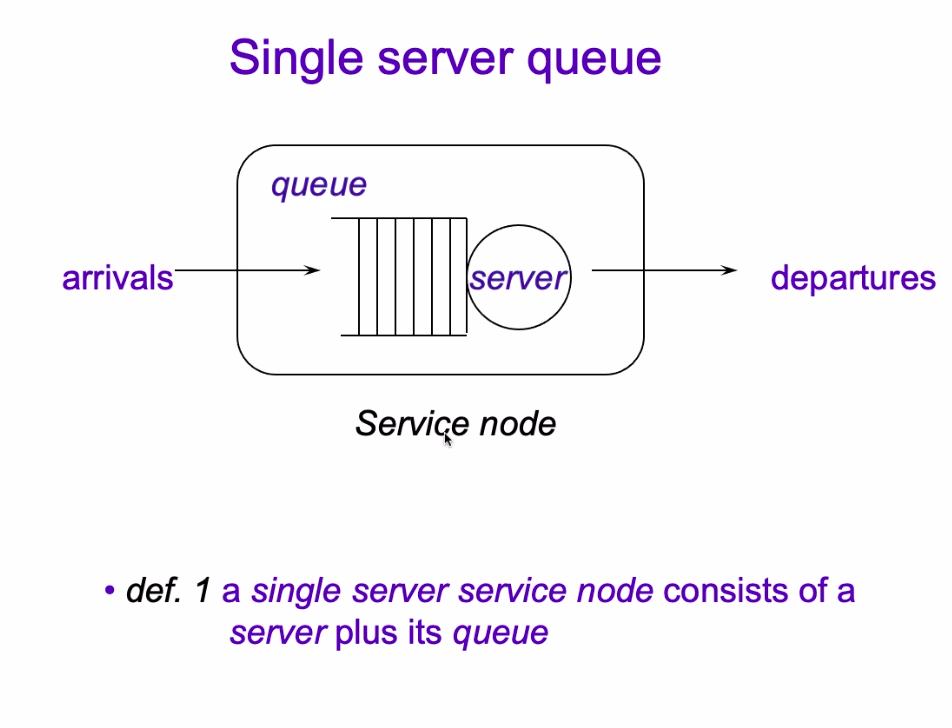
\includegraphics[scale=0.2]{images/PMCSN-1.png}\\
Ho due parti:
\begin{itemize}
\item server: la risorsa che deve essere assegnata, è singolo perché in questo modello semplice si assume che è possibile servire una singola richiesta
\item queue: mantiene tutte le altre richieste che possono arrivare per il servizio. Quando termina il servizio, viene scelta la prima richiesta in coda
\end{itemize}
Spesso si assume che le richieste per il servizio arrivino ad istanti random: non c'è correlazione tra gli istanti di arrivo delle richieste. Questa caratteristica modella bene la stragrande maggioranza dei processi di arrivo.\\ Inoltre, si assume che la coda di buffer sia infinita (non ho la linea nera alla fine), ma spesso si è interessati alla loss probability: dato che la coda è finita, voglio conoscere la probabilità che nel momento in cui una richiesta arriva questa venga rifiutata in quanto non può essere messa in attesa. Ad esempio, in comunicazione tale probabilità di perdita è proprio il livello di connettività offerto da una rete.\\ 
\subsection{Definizioni}
La coda è un elemento importante di questa astrazione, è l'area di buffer in cui possono attendere i job che non possono essere serviti. Bisognerà decidere la politica di scelta con cui si serve il job successivo, una volta che ha finito quello corrente.\\ Disciplina di scheduling è quell'algoritmo secondo il quale si sceglie un job dalla coda:
\begin{itemize}
\item FIFO: serve il job arrivato per prima nel sistema: se arriva un job ed il servizio non è disponibile, questo prende la prima posizione in coda. Un secondo job andrà dietro l'ultimo entrato, quindi gli istanti di partenza dal server saranno ordinati nello stesso modo con cui sono stati ordinati gli istanti di arrivo
\item LIFO: opposto della FIFO, i job vengono presi a partire dall'ultima posizione della coda
\item random
\item priority: i job non sono tutti uguali per il sistema, alcuni hanno valore maggiore di altri. Può esserci un criterio di priorità secondo il quale vengono scelti sempre (se ci sono) i job di priorità più alta
\item processor sharing: rappresentazione ideale di quello che succede in un sistema time-sharing, in cui ad ogni job è assegnato un quanto di tempo per usare la risorsa. TCP ad esempio divide la banda fra i diversi job che sono attivi in un certo istante di tempo, quindi tale disciplina prevede la condivisione della capacità elaborativa (avendone assegnata $\frac{1}{n}$, se ho n job) come se fossero tutti attivi in simultanea
\end{itemize}
Si parla di job non-preemptive se un job che ha iniziato il servizio non può essere interrotto. Se invece il servizio è preemptive, allora questo può essere interrotto per dare il servente ad un job a priorità maggiore (nel caso di algoritmo a priority). Quindi, la processor sharing, avendo questo meccanismo, entra nella classe delle discipline preemptive.\\ Altra caratteristica è quella del servizio conservativo: potrebbe avere senso, nel caso in cui ci siano conoscenza della caratteristica del flusso di job che arrivano, che nel caso in cui server divenga vuoto questo non prende un job e lo manda in esecuzione perché è a conoscenza del fatto che sta arrivando un flusso prioritario.\\ Nel caso in cui un server rimanga in attesa senza fare nulla, si parla di server non conservative. Faremo l'ipotesi di serventi conservativi.
\subsubsection{Primo esempio: quanto conta lo scheduling}
10 job, conosco i 10 istanti di arrivo dei 10 job: 15 47 71 111 123 152 166 226 310 320 e questi job richiedono delle unità di tempo di servizio: 43 36 34 30 38 40 31 29 36 30.\\ Tempo di risposta di un centro: tempo che passa da quando la richiesta arriva al centro a quando parte. Lo scheduling può avere un effetto enorme sulle prestazioni: calcolo la media dei tempi di servizi (del campione) = 34.7\\ Calcolo inoltre la varianza = 20.21 Il tempo di risposta medio è 26.70: qual'è la caratteristica che inficia molto negativamente su tale valore? La variabilità: prendo il campione di 10 tempi ed aumento la variabilità sommando e sottraendo 20: 63 16 54 10 18 60 51 9 56 10. La media rimane uguale, ma la varianza aumenta moltissimo, passando da 20.21 a 504.21\\ Se invece cambio lo scheduling, ordinando i tempi di servizio in modo che arrivino in ordine decrescente di richiesta (o crescente nel caso opposto). Cosa accade: da un punto di vista di media e varianza, non cambia nulla, ma cambia in termini di tempo di risposta. Infatti, nel caso di ordine decrescente (servo dal più piccolo al più grande), i tempi di risposta diminuiscono di molto. Se faccio il contrario, ovvero servo in ordine decrescente, allora ho il caso peggiore: tutti hanno davanti a se job che occupano per più tempo di quello che chiedono.\\ L'algoritmo di scheduling non costa nulla, ma il modo in cui si schedula può agire molto sulle prestazioni. La variabilità è sempre un indice negativo a livello di prestazioni
\subsection{Altri esempi-applicabilità della modellazione}
Ho un rete, conosco i route dei pacchetti, la loro frequenza di arrivo, il tempo di trasmissione e la lunghezza dei collegamenti. Con la teoria delle code, possiamo conoscere:
\begin{itemize}
\item valor medio del tempo speso nel router i
\item la distribuzione dei pacchetti nella coda al router i
\item tempo totale medio per poter andare dal punto A al punto B
\end{itemize}
L'approccio modellistico è anche usato come tool di progettazione: so che un server subirà un carico, dal punto di vista degli arrivi, raddoppiato. Dobbiamo fare in modo che gli utenti non si rendano conto di questo raddoppio, quindi che i tempi rimangano simili. Di quanto va aumentata la capacità operativa della CPU del server per poter mantenere lo stesso tempo di risposta medio?\\ La soluzione che viene subito in mente è prendere una CPU con velocità doppia, ma in realtà serve meno del doppio se l'obiettivo è quello di mantenere gli stessi tempi di risposta.\\ È possibile rendersene conto anche analiticamente, questo evidenzia quanto a volte l'intuizione può portare dalla parte sbagliata.\\ Se sostituissi la CPU con una di potenza doppia, il tempo di risposta sarebbe dimezzato rispetto a quello del giorno prima, quello che succede è che il sistema dal punto di vista del carico che sopporta e della capacità di elaborazione rimane identico, ma come se fosse velocizzato di un fattore 2. Quindi, questo comporta un tempo di risposta che è la metà.\\ Supponiamo ora di cambiare anche lo scheduling: da FIFO passiamo a processor sharing. Cambiano le cose? No.\\ Supponiamo di avere un modello di un sistema batch con due server (carico fisso): ho 6 job che possono andare nel server 1 o 2, che sono identici.\\ 
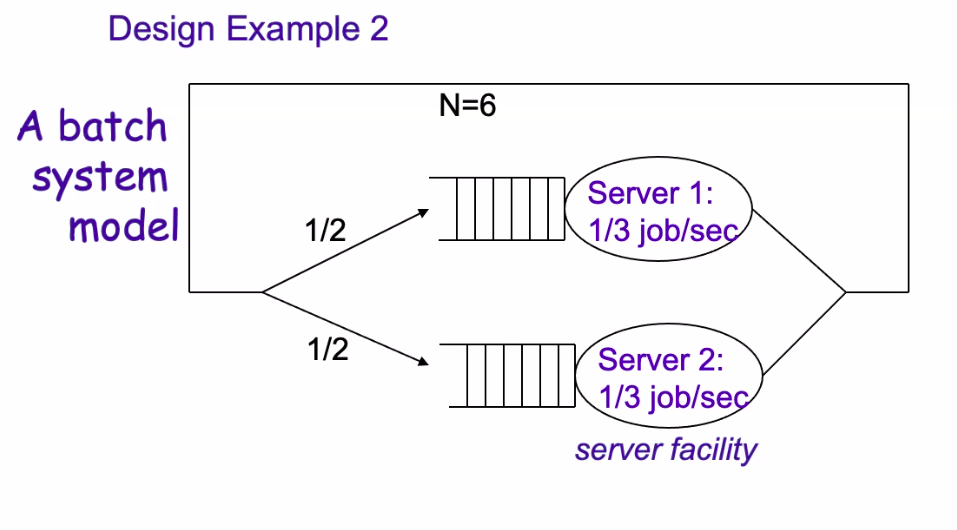
\includegraphics[scale=0.2]{images/PMCSN-2.png}\\
Supponiamo che il server 1 sia potenziato con uno che abbia il doppio della potenza, il tempo di risposta migliora? Ed il thoughput? Il miglioramento è poco e tende al nulla quanto più il numero di job del sistema cresce. Il problema è che nel sistema ho un bottleneck: posso migliorare il server quanto voglio, ma essendo il carico diviso a metà questo pesa nel calcolo della media (e noi guardiamo il calcolo della media). Se invece avessimo meno di 6 job, il miglioramento trascurabile diventa più apprezzabile? Sì, nel caso limite di uno stand alone job calcolerei la media come: 0.5$\cdot$tempo del server 1 (inverso della frequenza) + 0.5$\cdot$tempo di risposta del server 2.\\ Se invece il sistema fosse aperto (tempi di arrivo indipendenti dal completamento del servizio)? Cambia molto, migliorando uno dei due server, l'$\frac{1}{2}$ di arrivi che va nel server migliore ne risente, mentre prima c'era il bottleneck del server meno potente.\\ Altro esempio tipico, navigazione in Internet, vorrei sapere il tempo di risposta medio per una richiesta. Una situazione di questo tipo è spesso modellata, quando il numero di utenti è illimitato, infinit server; mentre se il numero è limitato sarà un centro ad un certo numero di serventi paralleli. Non ci sono code: quando arriva una richiesta c'è sempre un utente libero che aspetta la risposta.\\
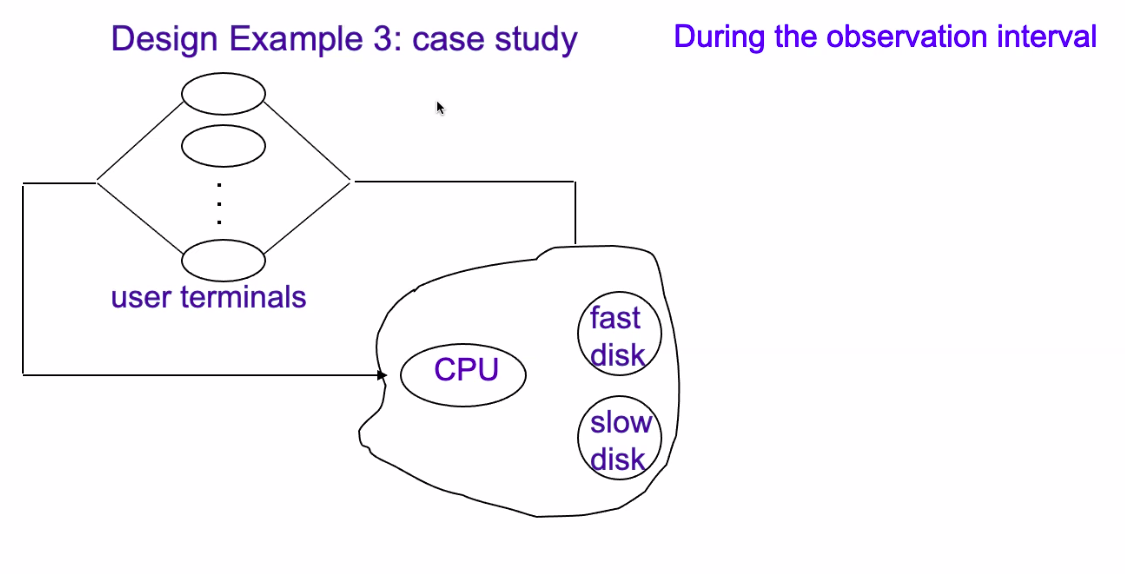
\includegraphics[scale=0.2]{images/PMCSN-3.png}\\
Osserviamo il sistema per un certo tempo (es T = 900 sec), possiamo sapere per ogni dispositivi:
\begin{itemize}
\item busy time: tempo in cui la risorsa è occupata
\item numero di completamenti, fatti nella finestra T
\item numero di completamenti del sistema
\item "think time" medio degli utenti: tempo per quanto aspettano gli utenti prima di lanciare un nuovo comando
\end{itemize}
Quale modifica è più effettiva per aumentare il throughput globale del sistema? Possiamo:
\begin{itemize}
\item prendere CPU con velocità doppia
\item fare load balancing dei due dischi
\item prendere un secondo disco veloce
\end{itemize}
Ancora una volta, la risposta è contro-intuitiva, l'approccio che è possibile usare per rispondere è l'analisi operazionale ed è "molto facile". Inoltre, è indipendente da assunzioni sulla distribuzione e non necessita di conoscere l'intera topologia della rete. Occorre però l'osservazione del sistema reale, per poter derivare le 3 quantità introdotte sopra.\\ Un altro problema molto interessante è il seguente: ho un certo budget, ad esempio in termini di potenza di calcolo ho $4\frac{job}{sec}$. Potrei avere questa potenza con 4 macchine da $1\frac{job}{sec}$ o una da $4\frac{job}{sec}$. Qui, si punta a minimizzare il tempo medio di risposta, ma occorre fare ipotesi. Partiamo dall'ipotesi che i job non siano preemtible. La soluzione migliore dipende dal carico, in particolare dalla variabilità del carico in termini di taglia del job.\\ Se c'è una alta variabilità, può accadere che un job piccolo venga bloccato da uno grande, quindi l'alternativa multi-server paralleli offre la possibilità di distribuire il carico di job piccoli in modo che non siano bloccati (ovviamente, tutti i confronti vanno fatti a parità di potenza computazionale). Viceversa, se la variabilità è bassa, conviene il singolo servente.\\ Se invece assumiamo che la classe sia preemtible, è sempre preferibile la configurazione ad un servente, perché possiamo togliere il job grande e mettere quello piccolo.\\ Il problema ha un'applicazione enorme, considerato che il server può rappresentare diverse risorse, problema è spesso il trade-off tra comprare una macchina più costosa che consuma di meno da un punto di vista energetico, oppure comprare un certo numero di macchine meno costose ma che dissipano più energia.
Un  altro problema molto diffuso riguarda il task assignment in una server farm o data center. Ho un dispatcher che si preoccupa di distribuire il workload fra diversi server. Ancora una volta, l'obiettivo del dispatcher può condizionare il tipo di politica adottata: per siti web, il dispatcher fa in modo di mantenere il carico di lavoro bilanciato fra i vari server. Nell'ambito dei super-computer la politica di bilanciamento può non essere utile.\\ Il modello è un certo numero di code ed il dispatcher davanti che deve distribuire fra le diverse code il carico che riceve. Facciamo delle assunzioni:
\begin{itemize}
\item server omogenei fra loro
\item risorsa singola per ciascun job, ogni richiesta che arriva al dispatcher userà una singola risorsa, sarebbe possibile che una richiesta possa chiedere l'uso di più di una risorsa, ma assumiamo di no.
\item scheduling delle code FIFO non-preemptible
\end{itemize}
Tra le politiche applicabili abbiamo:
\begin{itemize}
\item random: ogni job viene assegnato "lanciando una moneta equa"
\item round-robin: i job i-esimo va all'host $imodn$, dove n è il numero di host
\item shortest-queue: il dispatcher cerca di vedere il carico dell'host, manda il job all'host che ha il numero minimo di richieste
\item central-queue: unica coda, appena uno degli host diventa libero va sulla coda prende il primo job che trova
\item size-interval-task-assignment: assumiamo di conoscere la size delle richieste (in termini di carico di lavoro richiesto). I job vengono suddivisi in base alle size (si può anche avere una partizione più fine):
\begin{itemize}
\item short
\item medium
\item long
\end{itemize}
Si indirizzano i job in base alla taglia
\item least-work-left: si sceglie il server col carico minore, ogni job che arriva viene mandato al server dove a quell'istante di tempo c'è il minor carico, dove il carico è la somma delle size che si trovano in coda. Il server con valore minore sarà quello designato per ricevere il job
\end{itemize}
Le ultime due politiche sono size-based (non è sempre possibile conoscerla), mentre le altre no.\\ Supponiamo che si voglia scegliere la politica che comporta il tempo di risposta medio: dipende dalla variabilità della size:
\begin{itemize}
\item se poco variabili, la LWL comporta il tempo minimo
\item se molto variabili, la SITA comporta il tempo minimo
\end{itemize}
Quanto sarebbe quindi importante conoscere la size? In realtà, la maggior parte delle politiche usate non richiedono la conoscenza della size e si può dimostrare che in media la LWL è equivalente alla politica della central-queue: in qualche modo nella seconda politica si usa la nozione di size, in quanto il primo server che si libera all'istante di arrivo di un job è quello che aveva meno size.\\ Un'altra distinzione è fra classi di job preemptible e non: se non è preemptible non bisogna fare load balancing (non porta vantaggi) e bisogna fare altre considerazioni e studi. Il secondo è una open issue e dipende da cosa si vuole fare, se minimizzare il tempo di risposta o minimizzare il tempo di slow-down.\\ Nell'ipotesi che non vengano fatte assunzioni sulla taglia dei job e che ci siano job non-preemptive, è possibile dimostrare che finché non si mette in mezzo al taglia, è dimostrabile che non cambia nulla. Immagino ora di avere un algoritmo di scheduling FIFO preemptive, ovvero appena arriva un nuovo job ottiene subito il servizio. Per un carico che presenta almeno un minimo di variabilità si ha un miglioramento delle prestazioni enormi. Mentre invece, per un carico molto variabile, si ha un peggioramento delle prestazioni di quasi il doppio.
\section{Modelli analitici}
\subsection{Modelli a risorsa singola}
Ho una singola cosa, l'analisi guarda prevalentemente i valori medi (anche se potrei calcolare la distribuzione di probabilità)\\
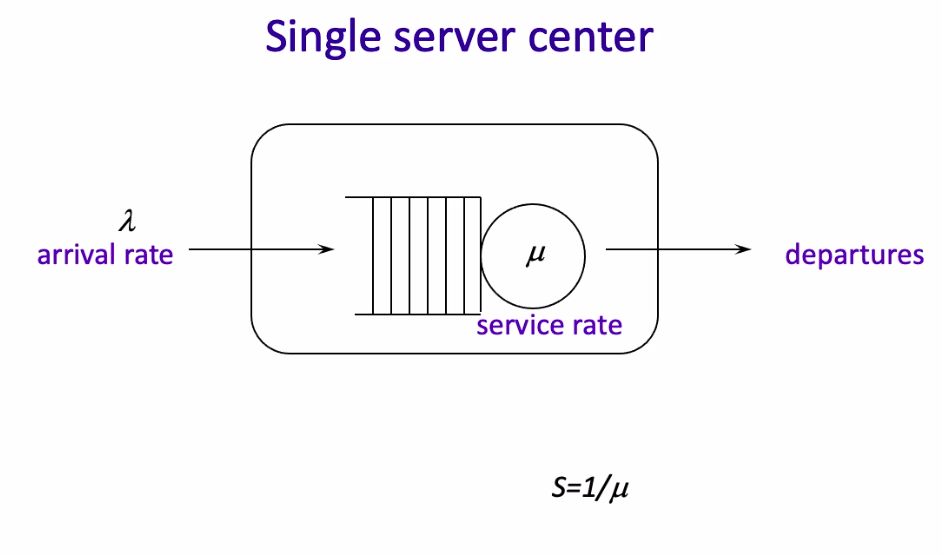
\includegraphics[scale=0.2]{images/PMCSN-4.png}\\
i parametri $\lambda$ e $\mu$ sono valori medi.\\ Si parte dalla definizione del modello concettuale (è sempre il primo passo che va fatto). Terminologia:
\begin{itemize}
\item S è il tempo di servizio ed è pari a $\frac{1}{\mu}$
\item $T_q$ è il tempo di coda
\item $T_s$ è il tempo nel sistema
\item $N_s$ è il numero nel sistema
\item $N_q$ è il numero in coda
\item U, $\rho$ è il numero nel servizio
\end{itemize}
Tipicamente, si considera il valore medio di tutte queste grandezze, un'altra misura importante, in  presenza di SLA e QoS, è P(\{$T_s > t$\}), che è la coda della distribuzione, mentre E(n)$_t$ è il numero medio di job serviti in un intervallo temporale t.\\ Quanto più $\lambda$ aumenta, tanto più cresceranno tutte le misure medie. Così come al crescere di $\mu$, che rappresenta la capacità di smaltire il traffico che arriva, le misure decresceranno.\\ Se rapportiamo E(n)$_t$ al tempo unitario 1, quindi E(n)$_1$ (possono essere secondi, minuti, ore etc...), stiamo guardando il throughput.\\ Altro fattore importante è l'utilizzazione, che ci da il rapporto tra il periodo di occupazione del servizio ed il tempo totale di osservazione.\\ Come definirlo matematicamente:\\
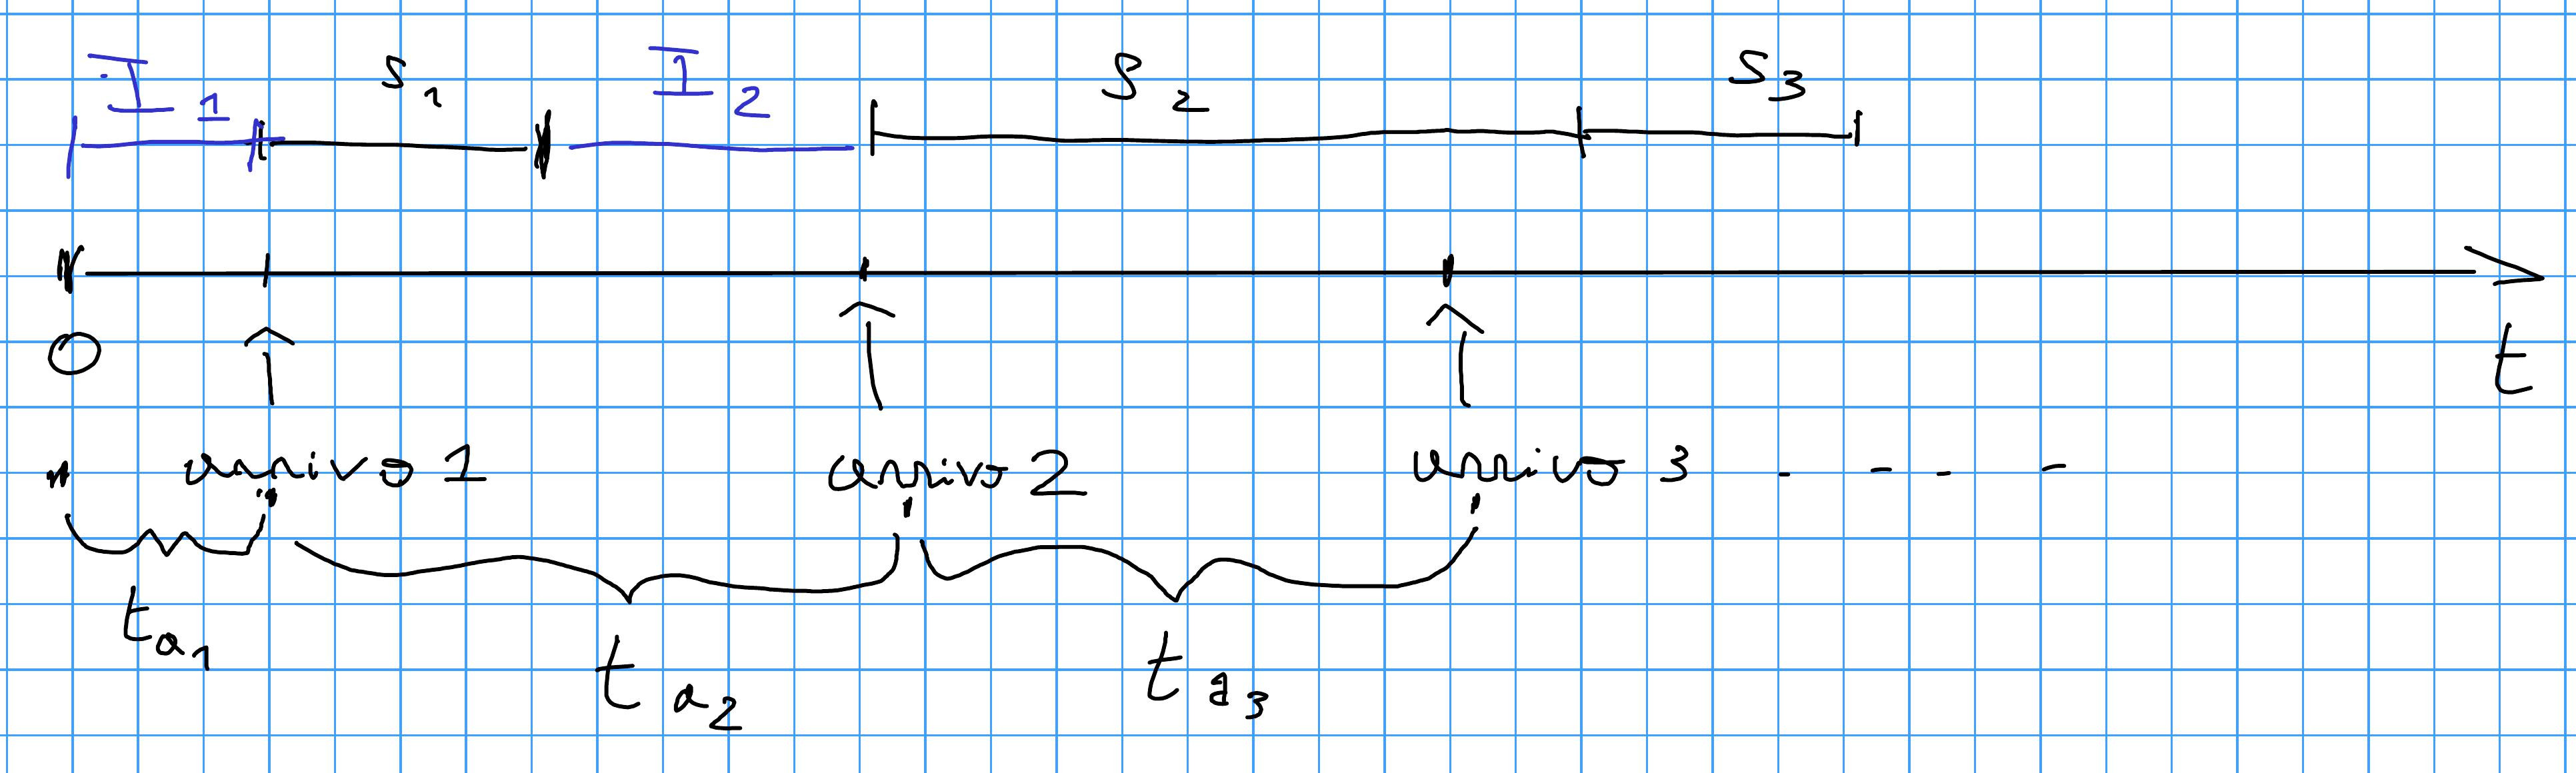
\includegraphics[scale=0.3]{images/PMCSN-5.jpeg}\\
Denotiamo con I gli intervalli in cui il servente è idle (non ha job in servizio), il tempo di occupazione totale sarà dato o da $t - \sum\limits_{i = 1}^{n} I_i$ oppure da $\sum\limits_{i = 1}^{n} s_i$.\\ Definiamo l'utilizzazione come $\rho = lim_{t-> \inf} \frac{B}{T}$.A questo punto, andiamo a sostituire i valori medi con le quantità per cui si considera il limite ottenendo $\cong \frac{E(\sum\limits_{i = 1}^{n} s_i)}{E(\sum\limits_{i=1}^{n} t_{a_i})}$.\\ Siccome gli $s_i$ sono indipendenti ed identicamente distribuite, così come le $t_{a_i}$, che sono tra l'altro esponenziali. Al di là della distribuzione, siccome hanno stessa media e stessa distribuzione, otteniamo $\frac{n\cdot E(s)}{n\cdot E(t_a)}$ = $\frac{E(s)}{E(t_a)}$ = $\frac{\lambda}{\mu}$ ed è anche $1 - P(n = 0)$, se n è il numero di job in coda. Quindi, possiamo dire che l'utilizzazione è il rapporto $\frac{frequenza\_di\_arrivo}{frequenza\_di\_servizio}$.\\ Possiamo anche dire che:
\begin{itemize}
\item $E(N_s) = E(N_q) + E(number\_in\_service)$, questo non è altro che $E(N_q) + \rho$
\end{itemize}
esempio:\\ 
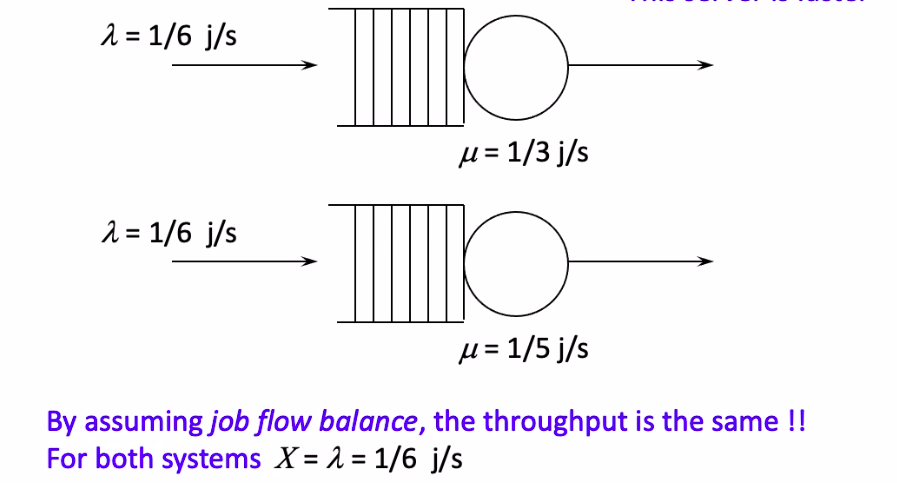
\includegraphics[scale=0.25]{images/PMCSN-6.png}
\\Il server più veloce è comunque utile, in quanto ci saranno dei tempi di risposta più brevi. Però, il minimizzare il tempo di risposta non è detto che migliori il thorughtput, come avviene in questo caso.\\ Se i centri sono in equilibrio stazionario, ovvero il flusso che entra è pari al flusso che esce (se $\lambda < \mu$ o $\rho < 1$), allora il thoughput è pari a $\lambda$. Se invece $\mu$ è maggiore di $\lambda$, il throughput è pari a $\mu$, ma questo vuole anche dire che la coda cresce indeterminatamente, perché il centro non riesce a smaltire le richieste in entrata.\\ Un altra metrica interessante è il tempo medio di servizio, definito in termini di C = della capacità operativa del server ($\frac{op}{s}$) e di Z = domanda media dei job (op): $\frac{E(Z)}{C}$.
\subsubsection{Server singolo a buffer finito}
Cosa accade nel caso di buffer finito: quando la coda è piena, l'arrivo si perde (c'è tutto un altro tema quando l'arrivo alla coda piena viene mantenuta dove c'è una certa area). Qual è in questo caso il throughput? Non è più $\lambda$ e cambia anche $\rho$ in quanto non entra $\lambda$ nella coda, bensì $\lambda'$. Dove c'è un buffer finito, c'è sempre l'equilibrio perché più di tanto non entra in coda, il sistema sarà sempre in grado di servire le richieste. Per poter calcolare il throughput, avremo bisogno dei processi di Markov, calcolare la probabilità di avere lo stato vuoto e quello saturo, la probabilità di perdita sarà la probabilità di avere la coda piena.
\subsection{Server a coda multipla}
Nel caso di un centro a servente singolo, vale che:
\[
N_s =
\begin{cases}
0 \\
1
\end{cases}
\]
se $N_q = 0$. Mentre $N_s = 1 + N_q \text{se } N_q > 0$. \\ Nel caso in cui abbiamo serventi multipli vale che:
\[
N_s = 
\begin{cases}
0 \\
1 \\
. \\
. \\
m \\
\end{cases}
\]
se $N_q = 0$, mentre invece $N_s = N_q + m$ se $N_q > 0$.\\
In questo caso, cambiano tutte le misure che abbiamo effettuato:
nell'immagine, consideriamo ogni servente identico\\
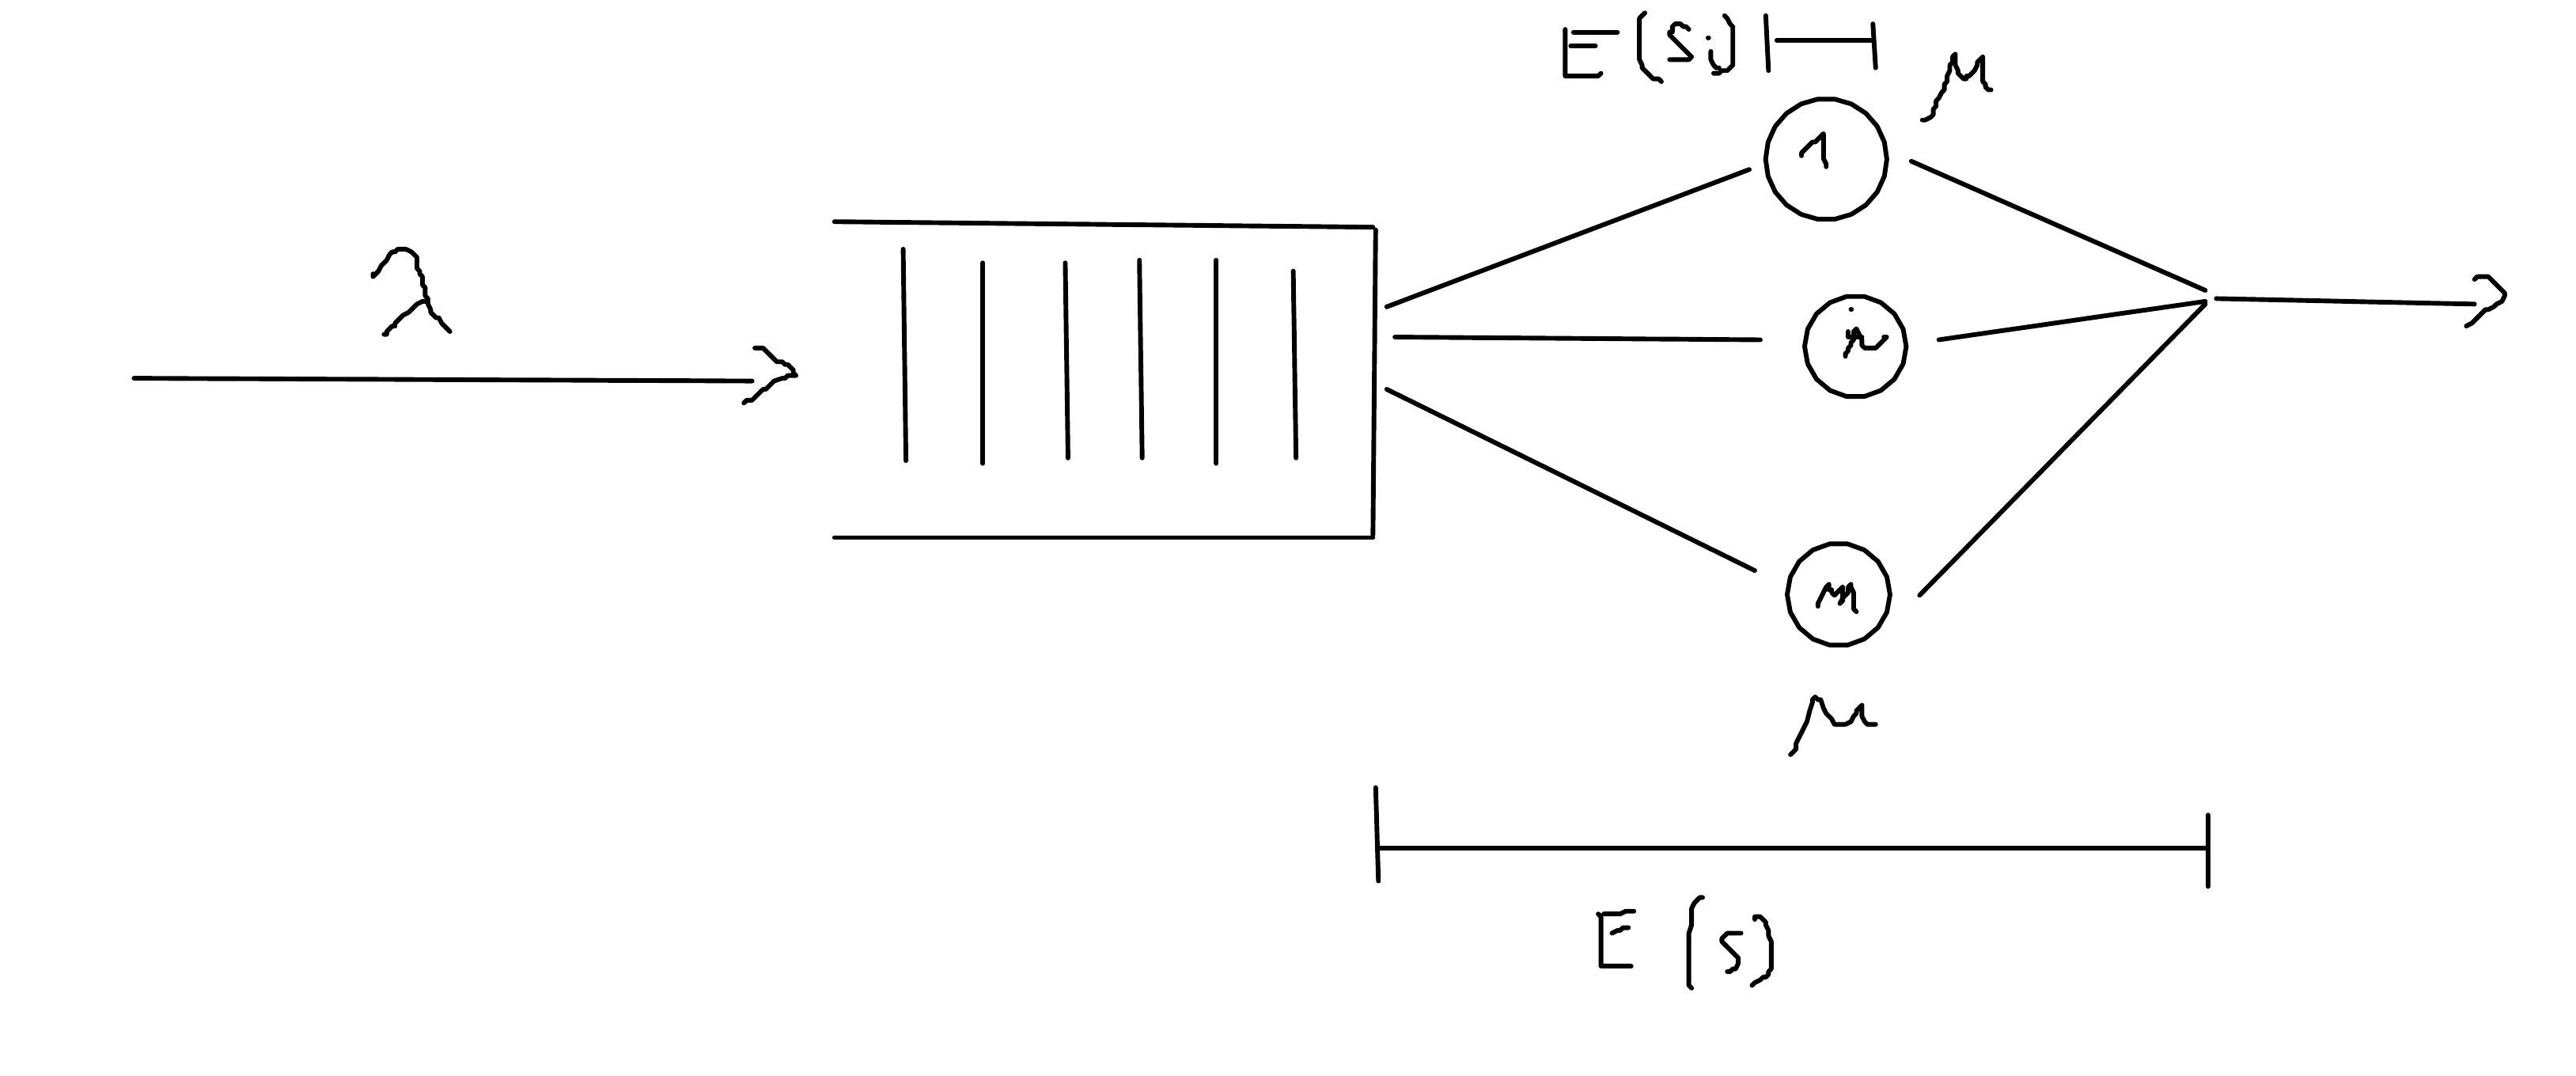
\includegraphics[scale=0.3]{images/PMCSN-903.jpeg}\\
il tempo di servizio medio, nel caso di un singolo server era $E(s)$, ora lo denotiamo con $E(s_i)$ e ci rappresenta il tempo che passa da quando un job si mette in coda a quando esce, quindi è il tempo di servizio medio su un server.\\ $E(s)$ è invece il tempo di servizio medio dall'istante in cui entra un job a quando esce un job (non per forza lo stesso), quindi è il tempo medio che occorre per liberare un server. I due tempi sono sicuramente diversi fra loro:
\begin{itemize}
\item $E(s_i) = \frac{1}{\mu}$
\item $E(s)$ è invece l'inverso del tasso globale, il multi-server ha una frequenza globale pari a $m\cdot \mu$, quindi $E(s) = \frac{1}{m\cdot \mu} = \frac{E(s_i)}{m}$
\end{itemize}
Per quando riguarda $E(N_s)$, abbiamo che:
\[
E(N_s) =
\begin{cases}
E(N_q) + \rho & \text{if } m = 1\\
E(N_q) + m\cdot \rho & \text{if } m > 1\\
\end{cases}
\]
Come viene definito $\rho$ nel caso del multi-server: in generale, sappiamo che $\rho \cong \frac{frequenza\_di\_ingresso}{max\_frequenza\_d'uscita}$, quindi andiamo a fare un prima distinzione fra:
\begin{itemize}
\item $\rho_i$, che è l'utilizzazione del singolo server
\item $\rho_{glob}$ che è l'utilizzazione globale del multi-server
\end{itemize}
Per $rho_i$, abbiamo che il tasso d'ingresso $\lambda$ viene diviso equamente su tutti gli m centri, quindi avremo $\rho_i = \frac{\lambda}{m\cdot \mu}$; per $\rho_{glob}$, il tasso d'ingresso è $\lambda$, ma la frequenza del multi-server è pari a $m\cdot \mu$, quindi abbiamo $\rho_{glob} = \frac{\lambda}{m\cdot \mu}$. Nonostante i due fattori di utilizzazione siano uguali, cambia il significato che hanno: se ad esempio consideriamo un $\rho = 0.7$, nel caso del singolo servente, e quindi di $\rho_i$, questo corrisponde al fatto che il centro sarà utilizzato per il $70\%$, per un periodo di osservazione lungo. Per quando riguarda invece $\rho_{glob}$, avere un valore di 0.7 vuol dire che in media il $70\%$ dei server saranno pieni.\\ Per quanto riguarda le relazioni medie introdotte in precedenza, abbiamo che:
\begin{itemize}
\item $E(T_s) = E(T_q) + E(s_i)$
\item $E(T_q) = f(\lambda, \rho, E(s))$
\end{itemize}
\subsection{Legge di Little}
La legge di Little permette di fare delle considerazioni sui valori medi di un sistema a code (anche per l'intera rete), vale sotto determinate assunzioni:
\begin{enumerate}
\item coda con disciplina FIFO
\item capacità del servente infinita
\item flussi bilanciati
\end{enumerate}
Nonostante ciò, è possibile applicare il teorema di Little anche se non valgono alcune delle ipotesi, ad esempio se il servente non ha capacità infinita o se per un periodo di tempo di osservazione del sistema non c'è il bilanciamento dei flussi.\\
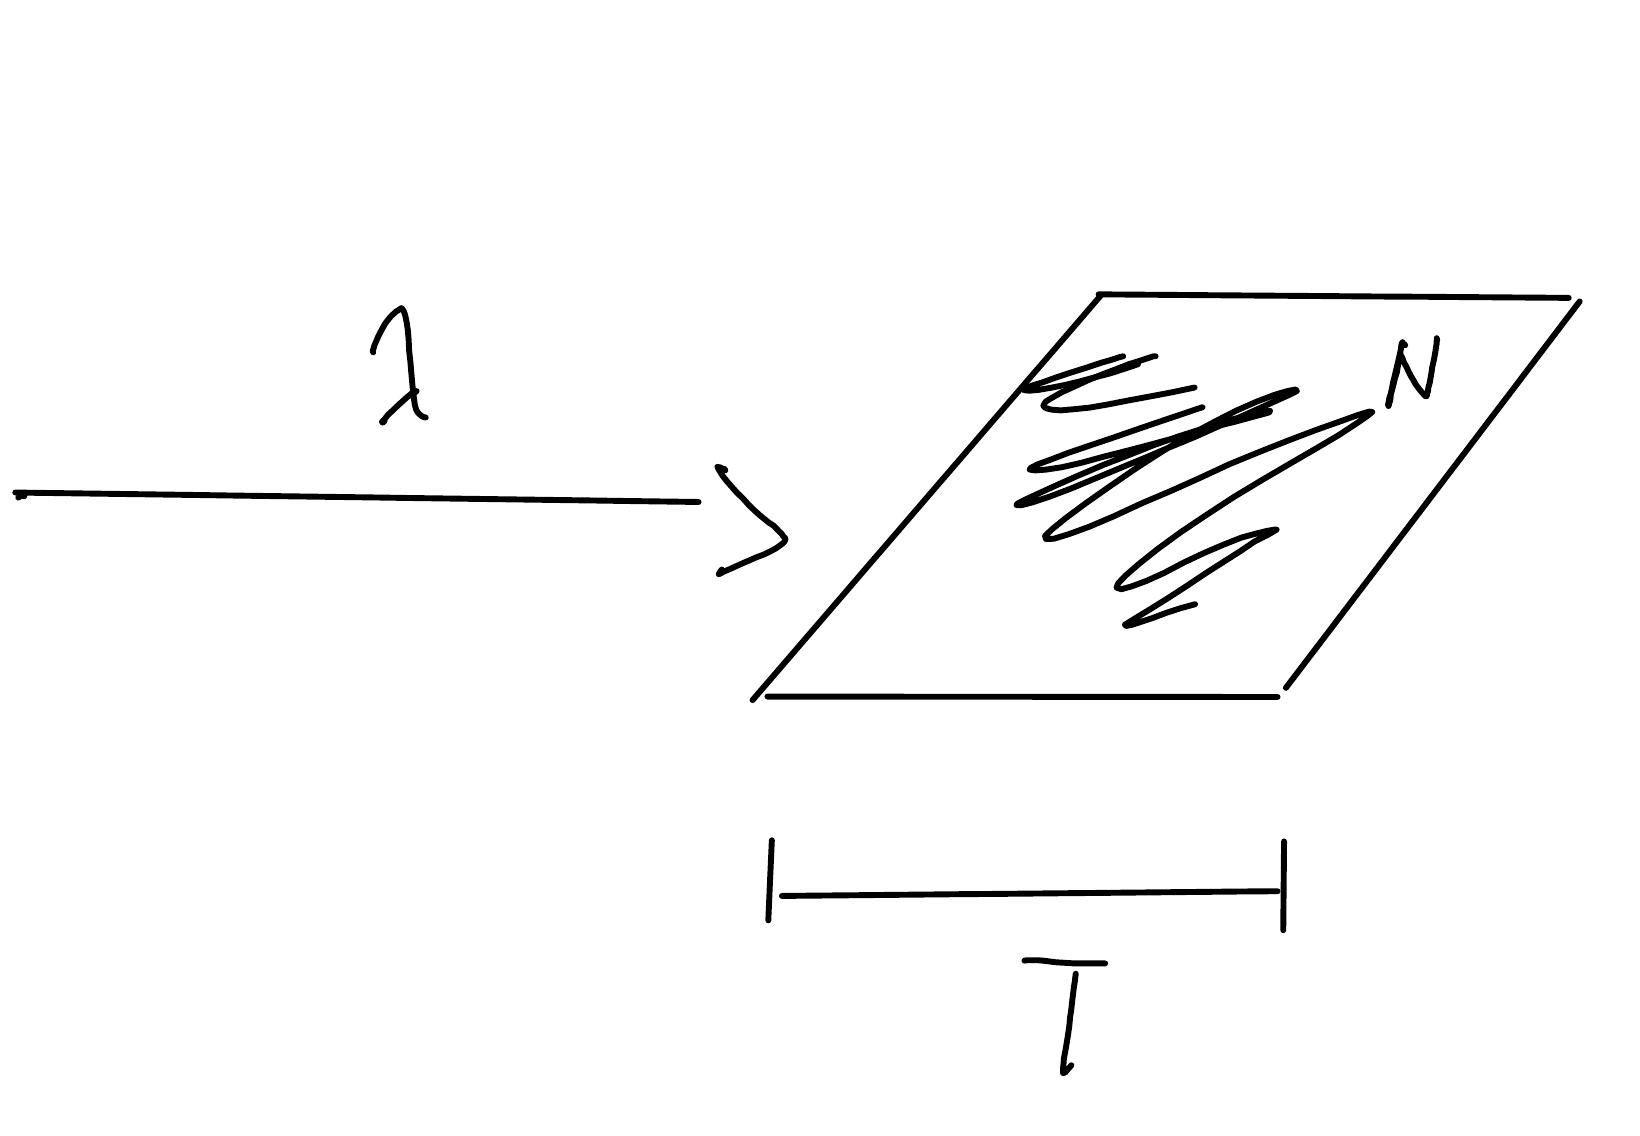
\includegraphics[scale=0.3]{images/PMCSN-903-1.jpeg}\\
\paragraph{Legge di Little:}sia $N$ il numero medio di popolazione in una "black box", $\lambda$ il tasso di arrivi medio e $T$ il tempo medio di percorrenza della box. Allora vale che $N = \lambda\cdot T$.\\ Possiamo ipotizzare che la black box sia qualunque coda:
\begin{itemize}
\item la coda + il servente: la legge ci fornisce $E(N_s) = \lambda\cdot E(T_s)$
\item la singola coda: $E(N_q) = \lambda\cdot E(T_q)$
\item il solo servente: $\rho = \lambda\cdot E(S)$
\item l'intera rete: $N = \lambda\cdot T$
\end{itemize}
È quindi possibile riscrivere tutte le relazioni trovate in precedenza per servente singolo e multi-server in funzione della legge di Little, ad esempio per il singolo centro:
\begin{enumerate}
\item $E(N_s) = \lambda\cdot E(T_s)$
\item $E(N_q) = \lambda\cdot E(T_q)$
\end{enumerate}
e vale lo stesso per il multi-server\\
\subsection{Risultati del modello analitico}
Abbiamo visto alcune relazioni per i valori medi, riscritte anche con la legge di Little. Le soluzioni note partono tutte da $E(N_q)$, cominciamo con il servente singolo.
\paragraph{Notazione di Kendall}: notazione del tipo $A/S/m/B/N/D$, dove:
\begin{itemize}
\item A si riferisce alla distribuzione degli inter-arrivi
\item S alla distribuzione del servizio
\item m al n° server
\item B alla capacità della coda
\item N alla taglia della popolazione
\item D alla disciplina della coda
\end{itemize}
Le distribuzioni più classiche sono $D, M. E_k, H_2, G$. \\ Per ora assumiamo scheduling astratto e non preemptive, quindi FIFO, LIFO non -preemptive, Random. Sembrerebbe che la FIFO, poiché rispetta l'ordine di arrivo, potrebbe essere quella che produce il tempo di risposta minimo (in quanto segue l'ordine di arrivo delle richieste), viceversa con la LIFO sembrerebbe che i job si vedano sempre bloccati da altri con tempi maggiori.\\ Ma tutte le politiche danno lo stesso \textbf{tempo di risposta medio}.\\ La notazione che utilizzeremo sarà $M/G/1$ con scheduling astratto.
\paragraph{Equazione di Khinchin Pollaczek (1930):}da una espressione per il livello di congestione nella coda, ovvero quanti job in media si trovano nella coda. $E(N_q) = \frac{\rho^2}{2\cdot (1 - \rho)} \cdot [1 + \frac{\sigma^2(S)}{E(S)^2}]$. $C^2 = \frac{\sigma^2(S)}{E(S)^2}$ vuol dire che la variabilità incide moltissimo sulle prestazioni: $C^2$ misura la dispersione dei tempi di servizio attorno alla media, quindi potrei avere distribuzioni con la stessa media, ma se la varianza è differente le cose cambiano di molto (rivedi esempi di introduzione. La congestione della coda, ovvero la popolazione media, è proporzionale a $C^2$; la formula fa riferimento ad un sistema all'equilibrio e tutti i risultati analitici fanno riferimento a sistemi all'equilibrio (o $E(N_q) -> \infty$.
\subsection{Distribuzioni a fasi}
Facciamo la distinzione fra le diverse distribuzioni a fasi,ovvero in cui si combinano più fasi esponenziali per modellare il tempo di servizio, \textbf{consideriamo sempre un solo servente, che serve un solo job}:
\begin{itemize}
\item esponenziale: il tempo di servizio che viene caratterizzato da una fase, tasso $\mu$
\item k-Erlang: il tempo di servizio che viene caratterizzato con la k-Erlang è la successione di k tempi, dove ciascuna fase è esponenziale. Le fasi sono uguali fra di loro, con tasso $\mu k$, un job che prende servizio termina tutte le k fasi e poi esce
\item distribuzione iper-esponenziale a 2 fasi: c'è una alternanza con probabilità $p$ fra due tempi esponenziali. I due tempi sono legati da una relazione, che dipende da $p$:
\begin{itemize}
\item tasso del 1° stadio è $2p\mu$
\item 2° stadio ha tasso $2(1-p)\mu$
\end{itemize}
quindi cambieranno le frequenze di servizio.\\ Quando $p = 0.5$, i due stadi sono equiprobabili, hanno entrambi tasso $\mu$, quindi l'iper-esponenziale diventa una esponenziale. Tanto più $p$ si allontana da 0.5, tanto più cresce la variabilità fra i due diversi possibili tempi
\item distribuzione di Cox: può modellare qualsiasi distribuzione. Può avere un numero arbitrario di fasi, ciascuna di esse è esponenziale ma al contrario della Erlang, dopo ciascuna fase possono accadere due cose (esclusa l'ultima fase):
\begin{itemize}
\item o si esce, questo accade nella fase i con probabilità $b_i$
\item o si passa all fase successiva e questo accade nella fase i con probabilità $a_i$
\end{itemize}
ovviamente devono valere le classiche regole, ovvero $a_i = 1 - b_i,  \forall i$ ed inoltre per lo stato finale k abbiamo $b_k =1, a_k = 0$.
\end{itemize}
Riscrivendo la KP in termini di $C^2$, otteniamo $E(N_q) = \frac{\rho^2}{2\cdot (1 - \rho)} \cdot [1 + C^2]$, dove $C^2$ dipende dalla distribuzione :
\begin{itemize}
\item D: $C^2 -> 0$
\item $E_k$: $C^2 = 1 + \frac{1}{k}, k \geq 1$
\item M: $C^2 = 1$
\item $H_2$: $C^2 = g(p) = \frac{1}{2\cdot p\cdot(1-p)} - 1$. Per $p = 0.5$, riotteniamo la $C^2$ di una M, mentre al crescere di $p$ cresce anche il termine $C^2$.
\end{itemize}
esempio: utilizziamo la KP per ricavare il tempo medio di attesa in coda. $E(T_q) = \frac{E(N_q)}{\lambda} = \frac{\rho^2}{\lambda\cdot 2\cdot(1-\rho)}\cdot(1 + C^2)$, scrivo uno dei $\rho$ al numeratore come $\lambda\cdot E(S)$ ed ottengo $\frac{\lambda\cdot E(S)\cdot \rho}{\lambda\cdot 2\cdot(1 - \rho)}\cdot (1 + C^2) = \frac{E(S)\cdot \rho}{1 - \rho}\cdot \frac{(1 + C^2)}{2}$. Anche per un fattore $\rho$ basso, ad esempio 0.5, il coefficiente $C^2$ per le heavy tails deve essere almeno pari a 25, quindi $\frac{1 + C^2}{2} = 13$, ovvero il tempo di attesa medio può diventare 13 volte il tempo di servizio.\\Nella tabella sono riportati in base al service time, $E(N_q)$ ed $E(T_q)$:\\\\
\begin{tabular}{ |c|c|c| }
\hline
Service time & $E(N_q)$ & $E(T_q)$\\
 & $\frac{p^2}{2\cdot (1 - \rho)} \cdot [1 + C^2]$ & $\frac{E(S)\cdot \rho}{1 - \rho}\cdot \frac{(1 + C^2)}{2}$\\
 &  & \\
Deterministic M/D/1 & $\frac{\rho^2}{2\cdot(1 - \rho)}$ & $\frac{\rho\cdot E(S)}{2\cdot(1 - \rho)}$\\
 &  & \\
Markovian M/M/1 & $\frac{\rho^2}{1 - \rho}$ & $\frac{\rho\cdot E(S)}{1 - \rho}$\\
 &  & \\
k-Erlang M/$E_k$/1 & $\frac{\rho^2}{2\cdot(1 - \rho)}\cdot (1 + \frac{1}{k})$ & $\frac{\rho\cdot E(S)}{2\cdot(1 - \rho)}\cdot (1 + \frac{1}{k})$\\
$\sigma^2(S) = \frac{E(S)}{k}$ &  & \\
 & & \\
Iper-esponenziale M/$H_2$/1 & $\frac{\rho^2}{2\cdot(1 - \rho)}\cdot(1 + g^2(p))$ & $\frac{\rho\cdot E(S)}{2\cdot(1 - \rho)}\cdot(1 + g(p))$\\ 
$\sigma^2(S) = E^2(S)\cdot g(p)$ &  &  \\
\hline
\end{tabular}\\\\ Al di là delle formule, è interessate notare come tutti i valori siano indipendenti da $C^2$.\\ esempio: richiamiamo l'esempio del provider che deve aumentare la potenza di calcolo per far si che gli utenti, nonostante il tasso di arrivi sia raddoppiato, sperimentino lo stesso tempo di risposta. Mostriamo in particolare come, se raddoppia la potenza il tempo di risposta risulta dimezzato:
\begin{itemize}
\item in partenza avevamo $\lambda, \mu, \rho$
\item ora, abbiamo $\lambda' = 2\cdot \lambda$, $\mu' = 2\cdot \mu$, ma $\rho' = \rho$
\end{itemize}
$E(S)'$ diviene pari ad $\frac{E(S)}{2}$, quindi ora consideriamo $E(T_s') = E(T_q') + E(S')$.Per quanto riguarda $E(T_q')$, vedendo le formule sopra, questo viene dimezzato (in quanto $E(S)$ è la metà), ed è quindi pari a $\frac{E(T_q)}{2}$. Quindi, abbiamo che $E(T_s') = \frac{E(T_q)}{2} + \frac{E(S)}{2} = \frac{E(T_s)}{2}$, quindi raddoppiando la potenza si dimezza il tempo di risposta.\\ Valgono le relazioni:
\begin{itemize}
\item $E(N_q)_D \leq E(N_q)_{E_k} \leq E(N_q)_M \leq E(N_q)_{H_2}$
\item $\sigma^2(N_q)_D \leq \sigma^2(N_q)_{E_k} \leq \sigma^2(N_q)_M \leq \sigma^2(N_q)_{H_2}$
\end{itemize}
C'è sensitività al tempo di servizio, visto che $E(N_s) + \rho$, vale lo stesso ordinamento. Con Little è possibile vedere la stessa cosa sui tempi, ma vale solo sulla media; per il momento del II ordine invece non vale.\\ Per quanto riguarda la sensitività allo scheduling, sono uguali sia media e varianza perché KP vale per ogni servizio astratto. Lo stesso vale per $E(N_s)$ ed ancora per $E(T_q)$, ma non per $\sigma^2(T_q)$ perché come abbiamo visto, lo scheduling conta.\\ Ad esempio, per uno scheduling LIFO, c'è la maggiore variabilità:\\
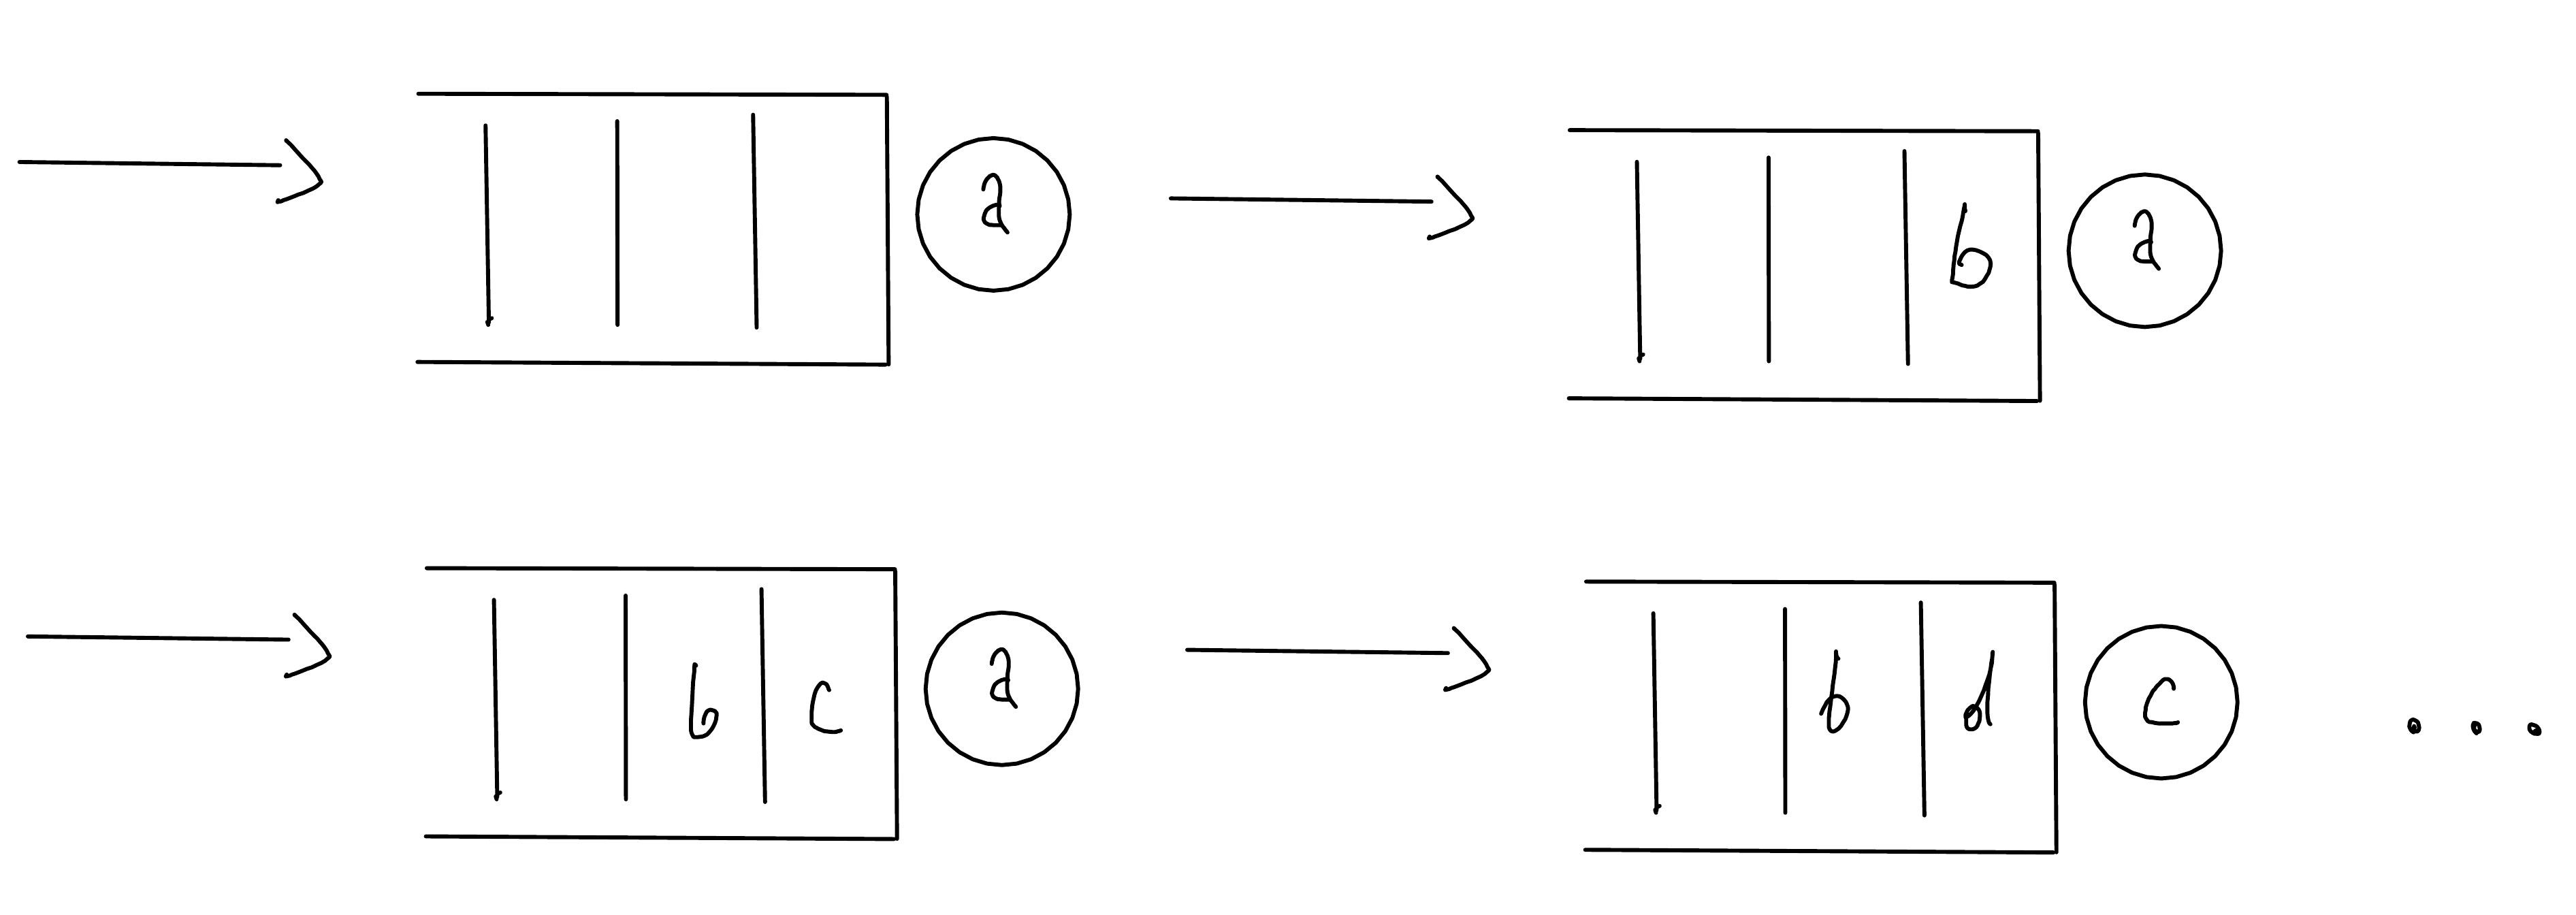
\includegraphics[scale=0.3]{images/PMCSN1003.jpeg}\\ in questo caso, b si vede arrivare sempre dei job e quindi risente del tempo di esecuzione di questi. L'esempio fa riferimento alla sola varianza, dato che nella media di tutti i possibili casi non conta, ed inoltre vale se $\rho$ è grande, in quanto questo corrisponde ad un'alta probabilità che al suo arrivo b trovi la coda piena.\\ Se consideriamo una esponenziale di parametro $\frac{1}{\mu}$:
\begin{itemize}
\item la k-Erlang ha $f_i(x) = k\mu e^{-k\mu x}$, media e varianza saranno divise per k
\item per l'iper-esponenziale, abbiamo che il singolo stadio  è una esponenziale: una sarà di param $2p \mu$ e l'altra $2(1 - p)\mu$. Per la media si fa la somma pesata delle due medie, e viene = $\frac{1}{\mu}$; per quanto riguarda la varianza abbiamo $\sigma(X) = g(p)(\frac{1}{\mu})^2$, dove $g(p) = \frac{1}{2p(1 - p)} - 1$ e tanto più ci allontaniamo da 0.5, tanto più p decresce e $g(p) -> \infty$
\item per distribuzioni generiche, abbiamo la distribuzione di Cox (può venire una distribuzione complessa). Ogni stadio è esponenziale di media $\frac{1}{\mu_i}$, dove i vari $\mu_i$ possono essere differenti e se $t_1, t_2, ..., t_k$ sono i tempi spesi in ciascuno stadio il tempo totale t è:
\begin{itemize}
\item t = $t_1$ con probabilità $b_1$
\item t = $t_1 + t_2$ con probabilità $a_1\cdot b_2$
\item t = $t_1 + t_2 + t_3$ con probabilità $a_1\cdot a_2 \cdot b_3$
\item ...
\end{itemize}
\end{itemize}
\subsubsection{Distribuzioni arbitrarie}
È sempre possibile trovare una distribuzione di Cox che approssima bene la funzione arbitraria, occorre guardare alla trasformata di Laplace e distinguere i casi in cui sia razionale o no:
\begin{itemize}
\item[a)] se è razionale, possiamo approssimare $C_k(t) = f(t)$ per un certo k, esatto o con una certa precisione nota
\item[b)] altrimenti, serve una $f(t) \approx g(t)$, in cui l'errore è noto ed a questo punto $C_k(t) \approx g(t)$, ma c'è un errore di sicuro
\end{itemize}
\subsubsection{Confronti}
Consideriamo un esempio con distribuzione esponenziale, $E(S) = 1s$, $\mu = 1 \frac{job}{s}$, se andiamo a graficare $E(T_q)$ in funzione di $\rho$ vediamo come dopo un valore di 0.7, la curva cresce velocemente a $\infty$.\\ Se confrontiamo con una k-Erlang (con k = 3), a parità di $E(S)$ (o il confronto non avrebbe senso), con $\mu = 2 \frac{job}{s}$, abbiamo come frequenza del singolo stadio $\frac{\mu}{k}$, $E(S_i) = \frac{0.5}{3} = 0.1666... s$ (tempo medio nello stato i) ed un $\sigma^2(S) = \frac{1}{k}\cdot (\frac{1}{\mu})^2 = 0.08333...$, un'esponenziale di stessa media avrebbe varianza pari a 0.25 (la varianza * 3).\\ Considerando infine una iper-esponenziale, con stessa $E(S)$, $\mu = 2 \frac{job}{s}$, $p = 0.2$ abbiamo che il primo stato ha un tasso pari a $2\cdot \rho\cdot \mu = 0.8 \frac{job}{s}$, mentre il secondo stato pari a $2\cdot(1 - \rho)\cdot \mu = 3.2 \frac{job}{s}$, quindi in media il 20\% del traffico riceve un servizio con tempo pari ad $\frac{1}{3.2}$, molto più basso di quello ricevuto in media dal restante 80\% del traffico.\\ esercizio:\\ un sistema TP accetta e processa uno stream di transazioni, mediate tramite un buffer grande.
\begin{itemize}
\item Le transazioni arrivano in modo random (distribuzione dei tempi di inter-arrivo random)\\
\item il server TP è in grado di servire transazioni ad un certo service rate
\end{itemize}
Se il tasso di arrivi e di servizio raddoppiano, sappiamo che il tempo di risposta dimezza. Supponiamo che $\lambda = 15 tps$ ed il tempo di servizio medio per transazione sia $E(S) = 58.37ms = 0.05837 s$. Cosa succede al tempo di risposta medio se la frequenza di arrivo cresce del 10\%?\\ $\lambda' = 16.5 tps$, $\rho = 87.56\%$, ora il $\rho' = 96.31\%$. Cosa possiamo dire su $E(S)$: siccome t. medio di servizio non è cambiato possiamo ragionare sul tempo medio di attesa. $E(T_q) = \frac{\rho}{1 - \rho}\cdot (\frac{C^2 + 1}{2})\cdot E(S)$, al cambiamento di $\rho$, i due termini che non vi dipendono non cambiano, quindi valutiamo il rapporto fra $E(T_q)$ ed $E(T_q')$: $\frac{E(T_q)}{E(T_q')} = \frac{\frac{\rho}{1 - \rho}}{\frac{\rho'}{1 - \rho'}} = \frac{7.0354}{26.1039} \simeq \frac{1}{3.7}$. Tempo di attesa quasi quadruplicato.
\subsection{Proprietà di mancanza di memoria e distribuzioni di probabilità}
La classe delle distribuzioni a fasi è molto importante, perché permette di modellare una distribuzione generale. La distribuzione esponenziale gode della memoryless property: informalmente, la RV non si ricorda del passato e si comporta come se fosse una variabile nuova, quindi il comportamento dipende solo dal presente.\\ esempi: supponiamo che la rv X sia il tempo trascorso in un negozio in un certo giorno della settimana dall'istante di apertura all'istante in cui entra il primo cliente. Oppure X sia il tempo da quando un server viene acceso a quando arriva la prima richiesta al server. La proprietà di mancanza di memoria fa un confronto fra la distribuzione di probabilità che valuta il fenomeno dall'istante 0 e la distribuzione che valuta il fenomeno aleatorio prima del momento in cui avviene per la prima volta un evento. Le due distribuzioni sono identiche.\\ Le uniche distribuzioni che soddisfano questa proprietà sono l'esponenziale e la geometrica; questa proprietà semplifica moltissimo l'analisi.\\ esempio: due utenti in fila alla posta, arriva un terzo utente. Qual è la probabilità che A sia l'ultimo ad uscire? $\frac{1}{2}$, uno fra B e C se ne andrà, quindi poi uscirà uno fra A ed il rimanente. Siccome i tempi di servizio sono esponenziali, la probabilità che finisca A o il rimanente è il $50\%$, non c'è influenza della storia passata.\\ Supponiamo di avere una v.a esponenziale di parametro $\frac{1}{\mu}$, quale è $P(X \leq t)$? = $1 - e^{-\mu t}$. Se condiziono invece rispetto al fatto che la v.a non ha terminato a $t_0$ e voglio scoprire la probabilità che termini a $t + t_0$, $X - t_0$ è \textbf{tempo di servizio rimanente}.\\ $P(X \leq t_0 + t | X > t_0) = \frac{P(X \leq t_0 + t \cap X > t_0)}{X > t_0} = \frac{P(X \leq t_0 + t) - P(X > t_0)}{P(X > t_0)} = ... = 1- e^{-\mu t}$
\subsubsection{Costante di decadimento dell'esponenziale}
L'esponenziale ha un'altra proprietà particolare: $f(t) = \lambda e^{-\lambda t}$, la calcolo in alcuni punti:
\begin{itemize}
\item $f(0) = \lambda$
\item $f(1) = \lambda e^{-\lambda} = f(0)e^{-\lambda}$
\item $f(2) = \lambda e^{-2\lambda} = f(1)e^{-\lambda}$
\item ...
\item $f(n) = f(n-1)e^{-\lambda}$
\end{itemize}
La media è $\frac{1}{\lambda}$, ed $f(\frac{1}{\lambda}) = \lambda e^{-1}$ ovvero: l'esponenziale parte da un punto che è il suo parametro e crolla, valutando f nella media $\frac{1}{\lambda}$ scopro che il suo valore iniziale è stato ridotto dell'$e^{-1}\%$, quindi la media è il tempo per ridurre la quantità iniziale del $1 - e^{-1} \%$. Questa viene detta costante di tempo ($\frac{1}{\lambda}$): se valuto la funzione di distribuzione nella media $\frac{1}{\lambda}: F(\frac{1}{\lambda}) = \int_{0}^{\frac{1}{\lambda}} f(t) dt = 1 - e^{-1} = 0.6321$.\\
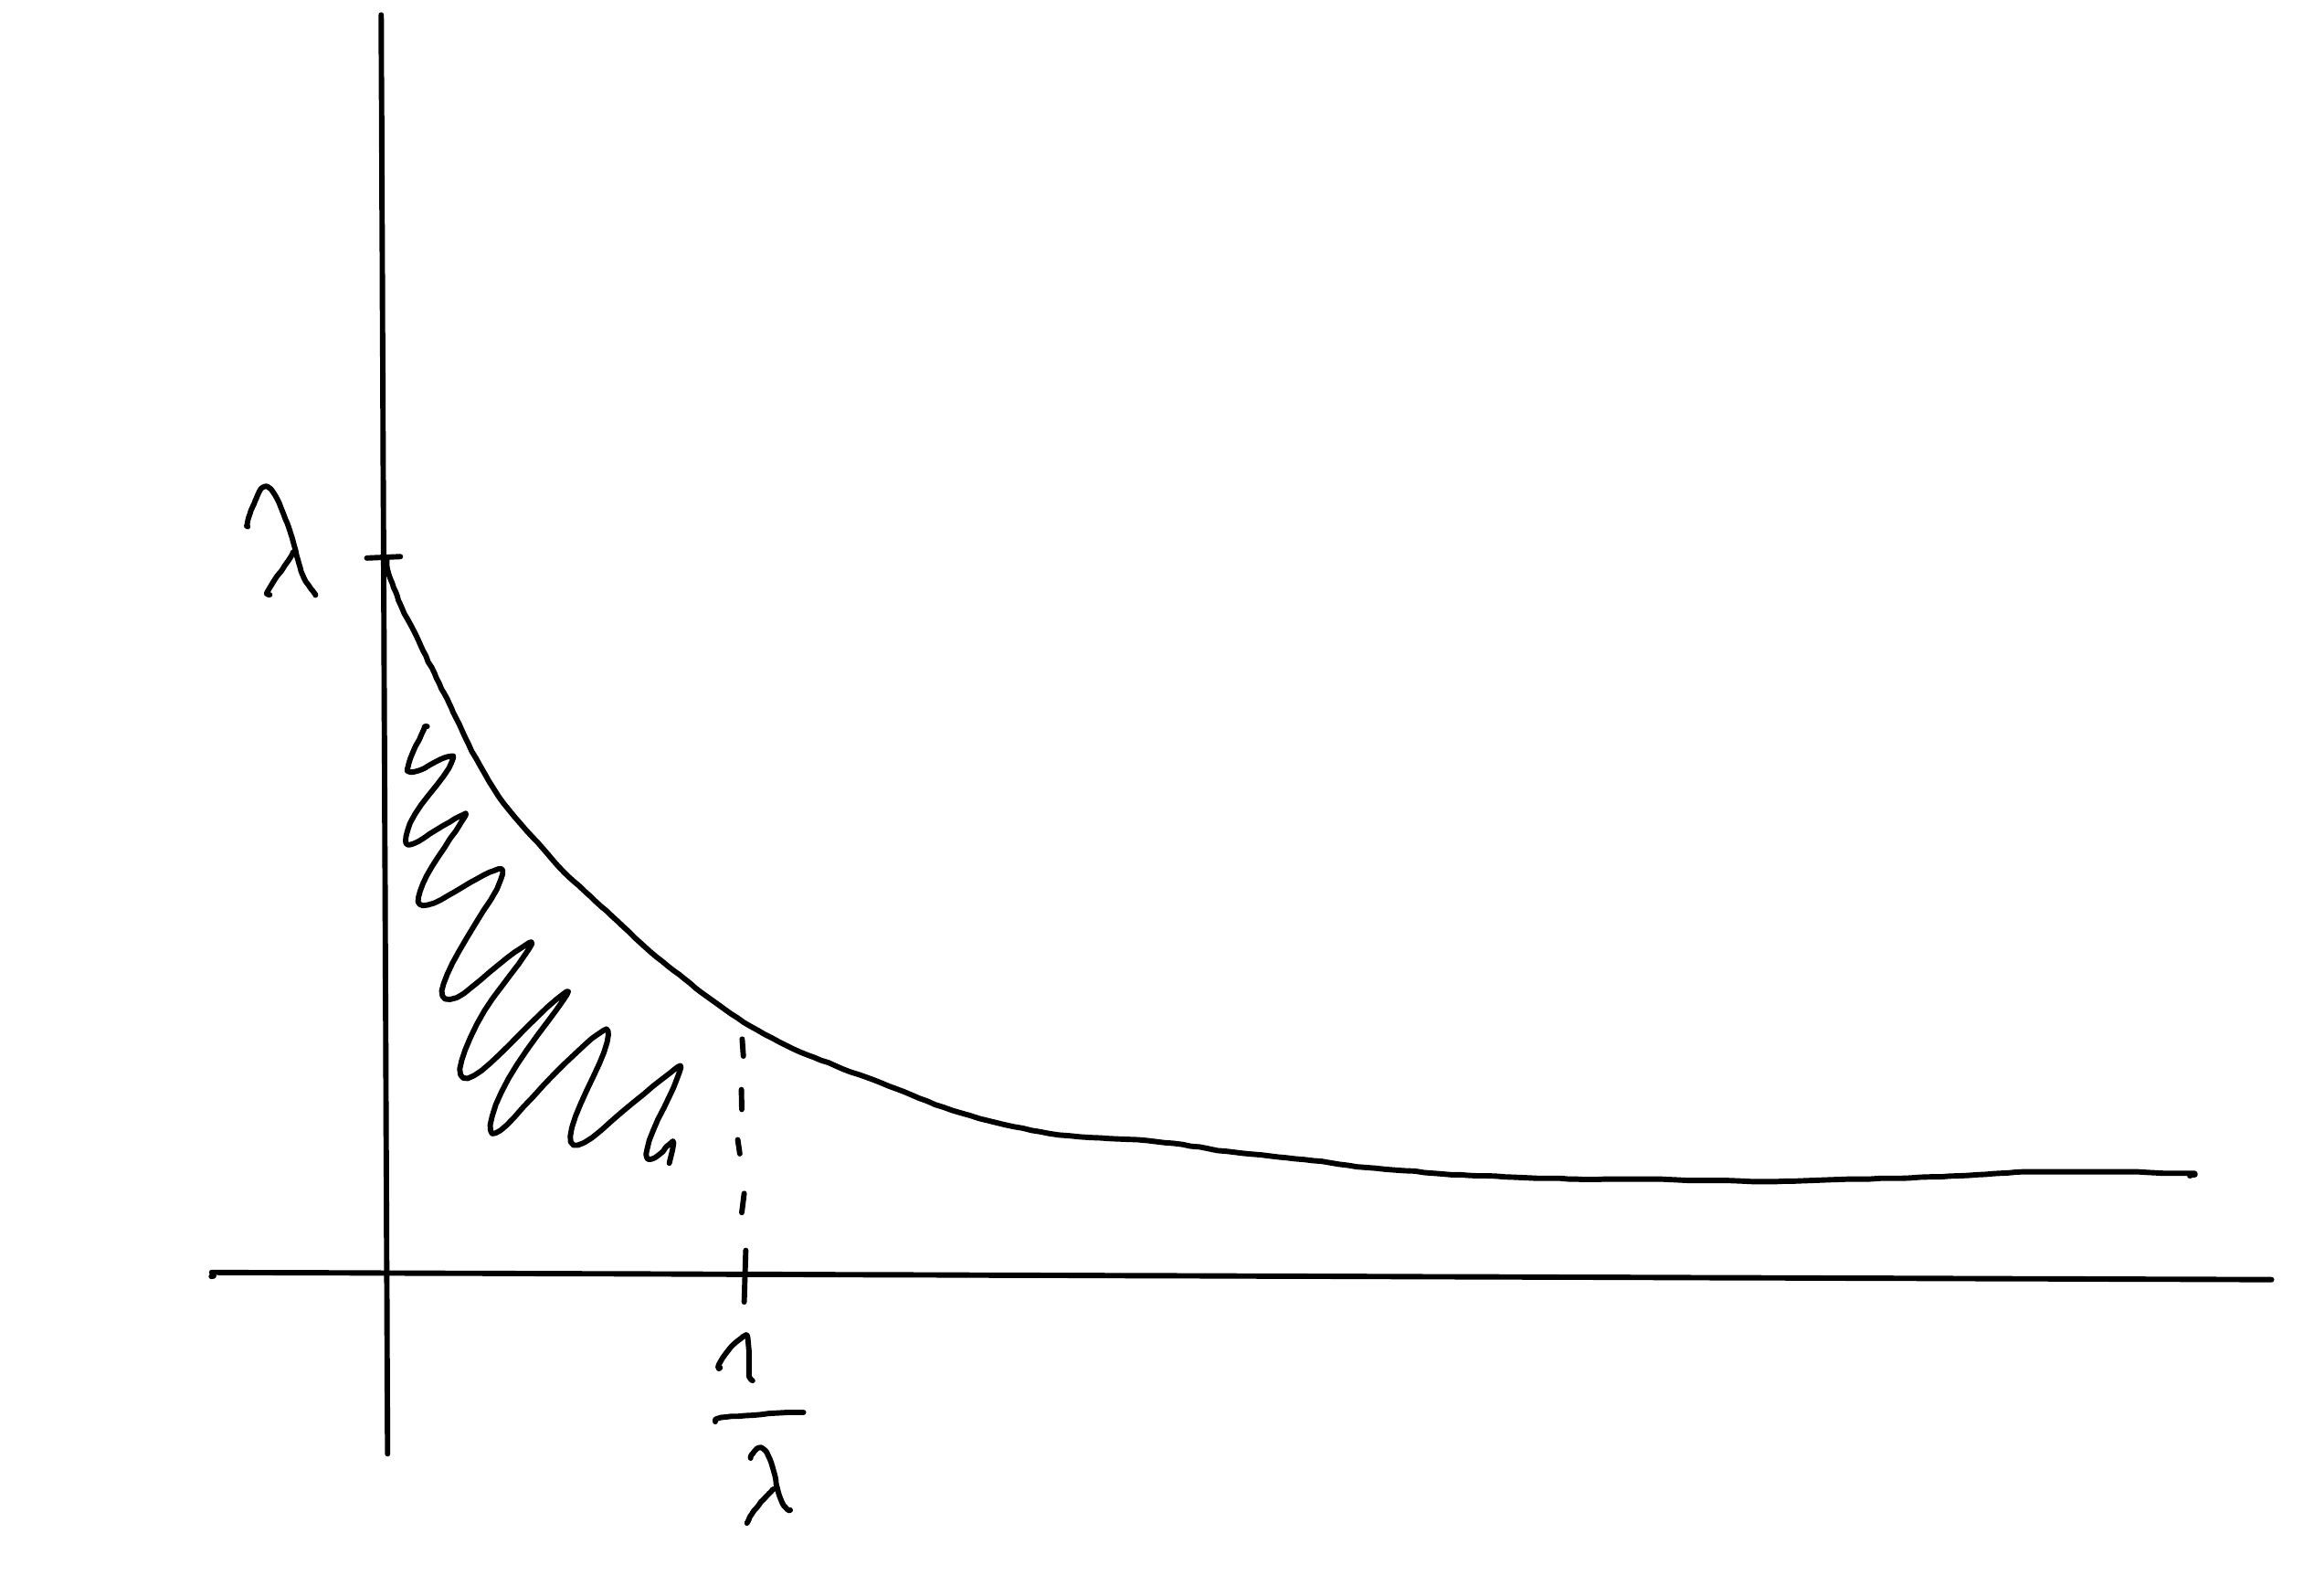
\includegraphics[scale=0.3]{images/PMCSN-exp.jpeg}\\
È indipendente da $\lambda$: qualunque sia la costante di tempo, questo equivale al tempo necessario affinché il valore iniziale si riduca di circa il $63 \%$.
\subsection{Memoryless come tempo di vita}
Una v.a X è detta memoryless se $P(X > s + t| X > s) = P(X > t), \forall s,t > 0$, ovvero il fatto che sia passato già un tempo s non conta nulla. esempio: sia X il tempo di vita di una lampadina. La memoryless direbbe che la probabilità che la lampadina duri ancora t secondi prima che si fulmini, dato che aveva funzionato per s secondi, è la stessa che la lampadina funzioni per almeno t.\\ Vediamo in termini di distribuzioni, non considerando la memoryless: considero tutte le distribuzioni per cui questo tempo di vita trascorso conta. Le distribuzioni per cui $P(X > s + t |X > s)$ decresce al crescere di s vengono dette a \textit{failure rate crescente}. Mentre, quelle per cui vale il contrario (ovvero al crescere di s la probabilità decresce), vengono dette a \textit{decreasing failure rate}.\\ esempi: il tempo di vita di una automobile è caratterizzato da un tempo di vita a increasing failure rate, nel caso chi ci riguarda di più:
\begin{itemize}
\item i tempi di vita dei job UNIX sono caratterizzati da distribuzioni decreasing failure rate: tanta più CPU ha usato un job, quanto più è probabile che ne debba usare altra
\item stesso vale per i chip: (test spesso eseguito per i chip) se non falliscono per un certo tempo, la probabilità di difetto è bassa (solitamente compaiono in un primo tempo).
\end{itemize}
\paragraph{Hazard rate function:}supponiamo di avere una v.a X continua con densità di probabilità $f(t)$ e funzione di distribuzione $F(t) = P{X < t}$, chiamiamo $r(t) = \frac{f(t)}{\bar{F}(t)}$, dove $\bar{F}(t)$ è il complementare della $F(t)$, consideriamo la probabilità che un oggetto di $t$ anni fallirà nei prossimi $dt$ secondi = $P(X \in (t, t + dt)|X > t) \approx \frac{f(t)dt}{\bar{F}(t)} = r(t)dt$, quindi la hazard rate function ci da il failure rate istantaneo.\\ Quando $r(t)$ è costante, allora la distribuzione è esponenziale.
\subsubsection{Importanza del tempo di vita rimamente}
Consideriamo un load balacing per la CPU in una rete di workstations: può essere utile migrare un job sulla workstation meno carica, per migliorare i tempi medi di risposta. Ma questo ha un costo, bisogna portarsi dietro lo stato del processo, ci sono due tipi di migrazioni:
\begin{itemize}
\item non-preemptive migration: re-alloca solo processi "nuovi", non ancora attivi
\item preemptive migration (active process migration): possibile migrare anche processi attivi
\end{itemize}
Ci poniamo delle domande: può essere utile la migrazione P, o basta la NP? E se scegliamo di usare la P, quale è una buona politica di migrazione (quale processo è meglio scegliere)?\\ Richiamiamo ancora una volta il lifetime, ricordiamo la terminologia:
\begin{itemize}
\item taglia di un job: domanda totale di CPU
\item vita di un job: utilizzo di CPU fino ad ora
\item tempo di vita di un job: richiesta totale di CPU di un job, dipende sia dalla capacità operativa che da quanto richiede (coincide sostanzialmente con la size
\item tempo di vita rimanente di un job: si riferisce ad un certo istante di tempo, la rimanente richiesta di CPU
\end{itemize}
Non per tutte le applicazioni è possibile conoscere tutti i termini, ma è sempre possibile su un sistema misurare quanta elaborazione è stata fatta, quindi è sempre possibile conoscere l'age (vita di un job).\\ 
\subsection{Distribuzioni di Pareto}
(vedi slide)
Vedo le raccolte dei tempi di vita di job Unix, sembrano distribuiti esponenzialmente ma non è così: per t=2 abbiamo una decrescenza di $\frac{1}{2}$, per t=4 $\frac{1}{4}$ etc..., classe delle distribuzioni di Pareto: $f(x) = \alpha \cdot k^{\alpha} \cdot x^{\alpha-1}$ con $k \leq x < \infty, 0 \leq \alpha \leq 2$, con code la cui misura è data da $\alpha$:
\begin{itemize}
\item $\alpha -> 0$, più variabilità e più pesantezza della coda
\item $\alpha -> 2$, il contrario
\end{itemize}
problema: hanno momento finito di ordine i sono se $\alpha > i$, quindi non possiamo valutarne la varianza.\\ Proprietà:
\begin{itemize}
\item sono a decreasing failure rate: più CPU viene usata, più continua ad usarne
\item hanno varianza infinita, la heavy tail property ci dice che una una minuscola frazione dei job molto grandi contribuisce alla metà del carico del sistema. Per esempio, con $\alpha = 1.1$, se migro i job grandi, tolgo la metà del carico dal sistema.
\end{itemize}
\subsubsection{Bounded Pareto}
L'infinito che limita la x si può togliere, si può facilmente trovare un limite finito molto grande alla size, si può passare alla classe bounded Pareto: $f(x) = \alpha \cdot x^{-\alpha - 1} \cdot \frac{k^{\alpha}}{1 - (\frac{k}{p})^{\alpha}}$ con $k \leq x \leq p, 0 < \alpha < 2$, tutti i momenti sono finiti.\\ $C^2 = 25$ è il minimo coefficiente di variazione misurato per distribuzioni di questo tipo, solitamente varia tra 25 e 49, quindi le prestazioni possono degradare moltissimo (con la variabilità), nel caso di distribuzione di questa classe.\\ Quindi, rispondendo alle due domande precedenti, la caratteristica del decreasing failure rate (quindi tutti i casi in cui l'applicazione viene ben modellata da questa caratteristica) ci porta a pensare che la migrazione è utile e può essere più sensato migrare i job vecchi. Sebbene i job vecchi potrebbe aver maturato uno stato più significativo di un job "giovane" (appena nato"), quel costo di migrazione verrà ammortizzato dal tempo in cui quel job continuerà a chiedere risorse di computazione.
\subsection{Risultati analitici ulteriori della KP}
Vediamo la KP nell'ottica del tempo di servizio rimanente. Ad un certo istante di tempo, la situazione di un server può essere la seguente:\\
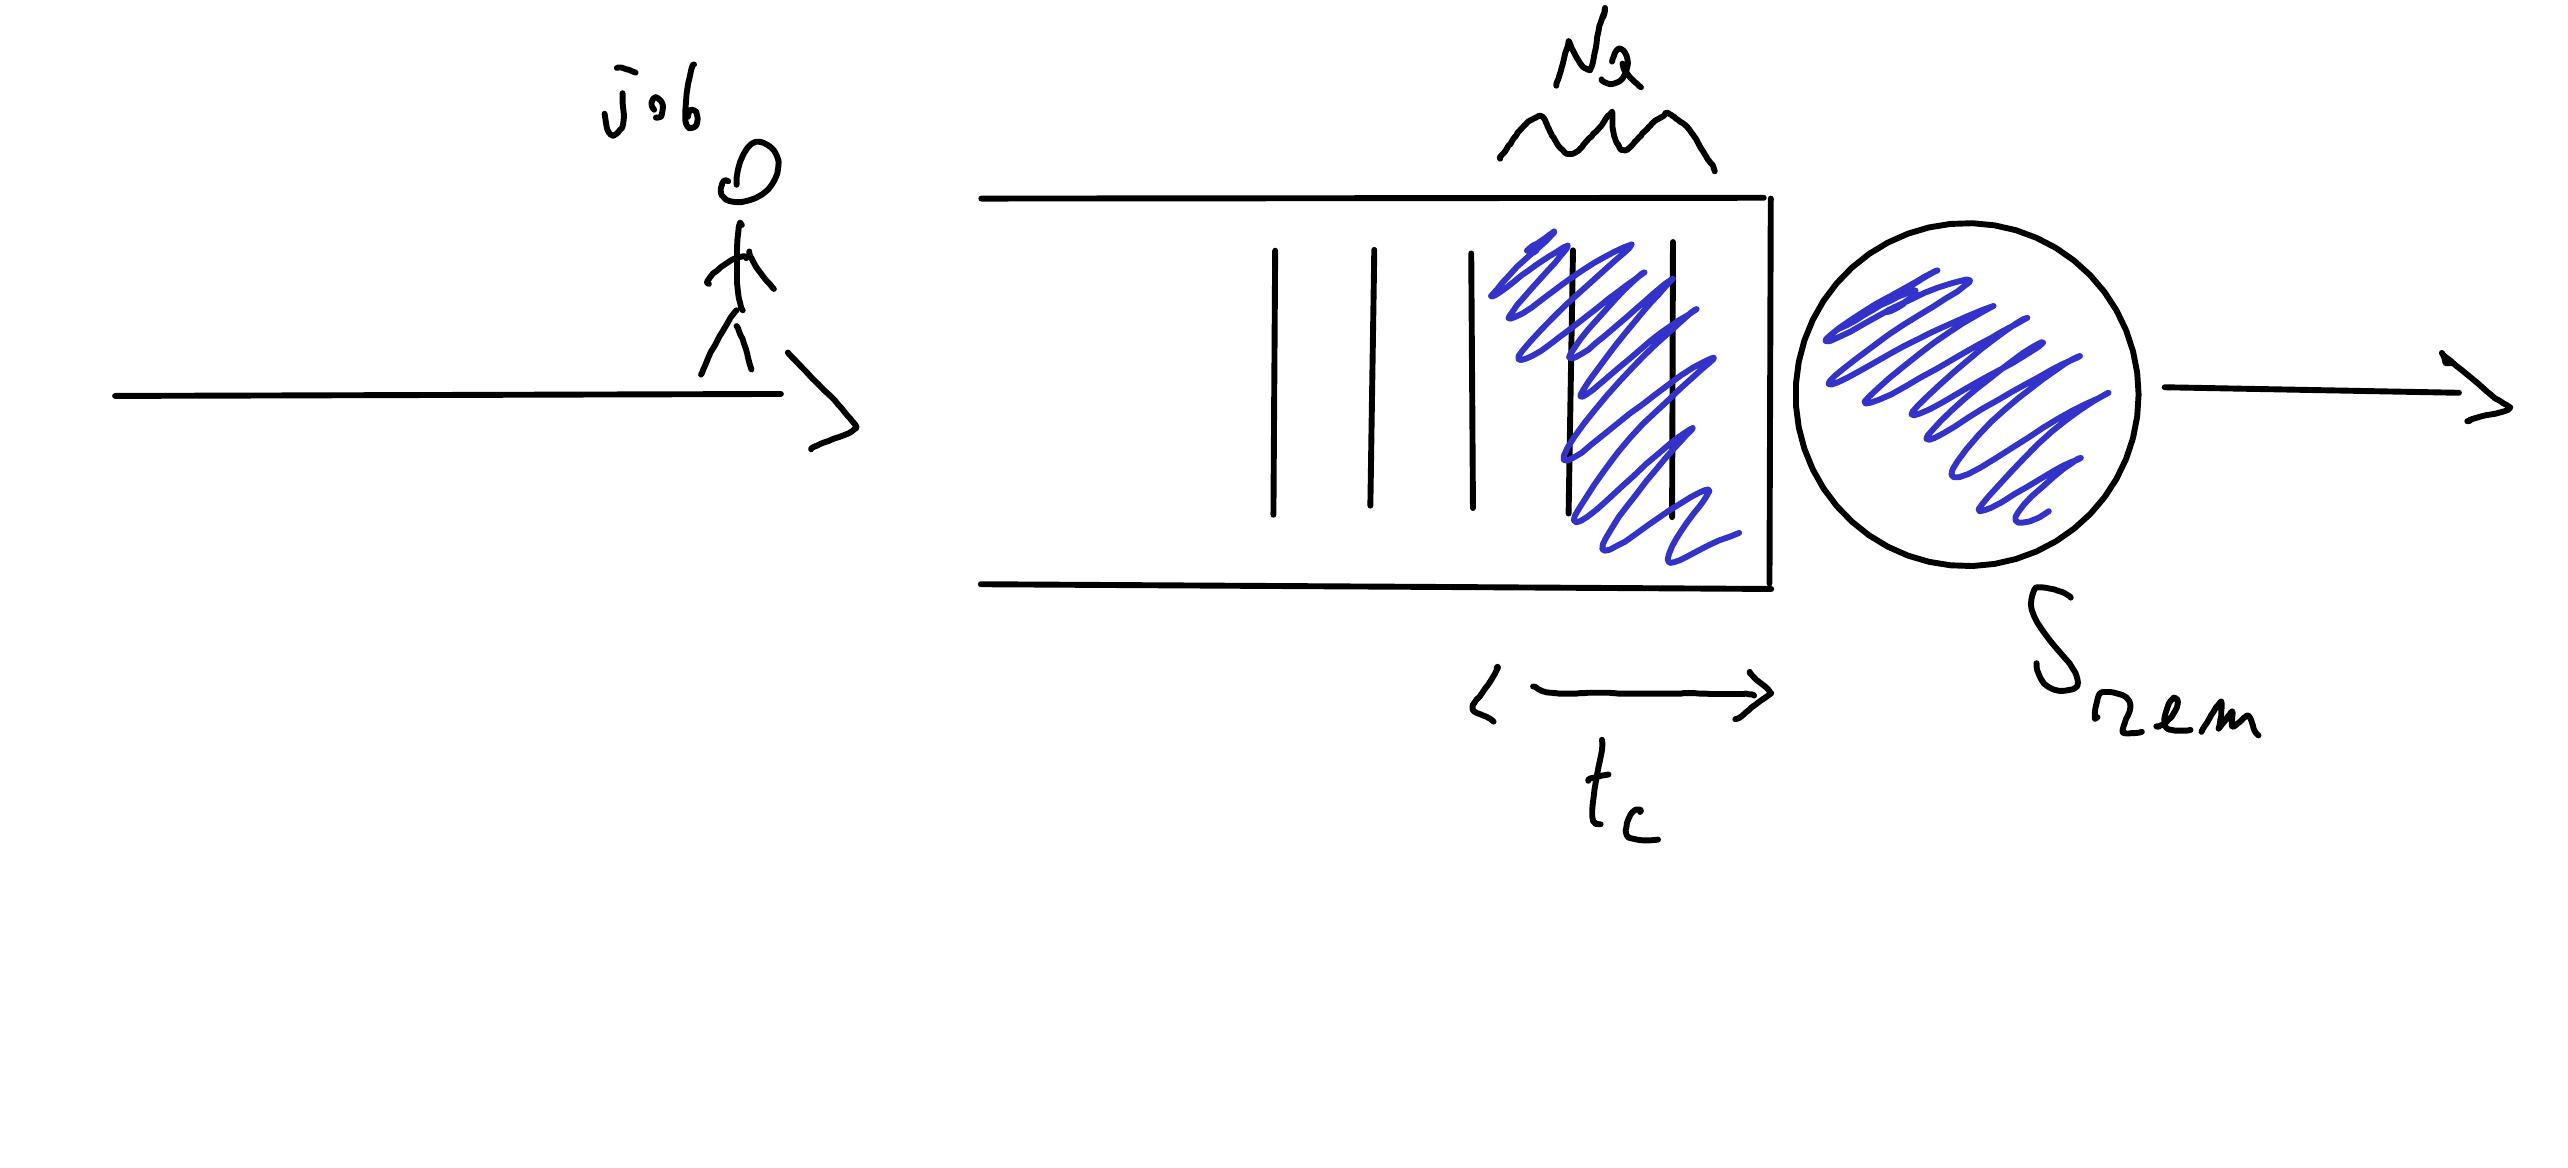
\includegraphics[scale=0.4]{images/PMCSN-1603.jpeg}\\
supponiamo che lo scheduling sia FIFO, il job che arriva dovrà attendere il tempo necessario ad elaborare i job nella coda ed il tempo di servizio rimanente del job in servizio. Il tempo di attesa sarà quindi una qualche combinazione $T_Q = t_c \oplus S_{rem}$, si può dimostrare che per \textbf{qualunque distribuzione} $E(S_{rem} = \frac{\lambda}{2}\cdot E(S^2)$. Nel caso dell'esponenziale, poiché $E(S^2) = 2\cdot E(S)^2 \rightarrow E(S_{rem}) = \frac{\lambda}{2}2E(S)^2 = E(S_{rem} = \rho E(S))$, quindi $E(T_Q) = \frac{\rho E(S)}{1 - \rho} = \frac{E(S_{rem})}{1 - \rho}$, quindi l'operazione per l'esponenziale è un prodotto di $E(S)$ con $\frac{1}{1 - \rho}$ (che non è il tempo per completare, \textbf{ma è un numero puro}).\\ Nel caso generale (KP): $E(T_Q) = \frac{\rho}{1 - \rho} \cdot \frac{C^2 + 1}{2}\cdot E(S) = \frac{1}{1 - \rho} [\frac{\sigma(S)^2}{E(S)^2} + 1]$ = $\frac{\rho}{2(1 - \rho)}\cdot[\frac{E(S^2) - E(S)^2}{E(S)^2} + 1] = \frac{\lambda E(S)}{2(1 - \rho)}[\frac{E(S^2)}{E(S)^2} - 1 + 1]$ = $\frac{\lambda}{2(1 - \rho)}[\frac{E(S^2)}{E(S)^2}]E(S)^2 = \frac{\lambda}{2}\cdot \frac{E(S^2)}{1 - \rho}$.\\ Il termine $\frac{1}{1 - \rho}$ rappresenta il fattore legato al $t_c$ (NON È UN TEMPO), siccome i due termini sono combinati con un prodotto:
\begin{itemize}
\item se uno è 0, il risultato è 0. Se $E(S_{rem}) = 0$, allora non c'è coda. Il job che arriva non deve attendere e viene subito servito
\item se uno è 1, abbiamo un invariante per il prodotto. Se il coefficiente $\frac{1}{1 - \rho}$ fosse 1, il job che arriva trova solo il job in servizio, quindi in pratica è come se non attendesse nulla
\end{itemize}
\paragraph{Tempo di risposta} per il tempo di risposta $E(T_S)$ abbiamo:
\begin{itemize}
\item M/G/1: $E(T_S) = E(T_Q) + E(S) = \frac{\frac{\lambda}{2} \cdot E(S^2)}{1 - \rho}$
\item M/M/1: $E(T_S) = \frac{\rho E(S)}{1 - \rho} + E(S) = \frac{E(S)}{1 - \rho}$.
\end{itemize}
\subsection{Scheduling astratto non-preemptive}
Riprendiamo le definizioni sullo scheduling, abbiamo dei risultati molto più forti di quelli della KP. Ricordiamo che: 
\paragraph{Definizione 1:}una politica prevede preemptive se un job può essere fermato durante la sua esecuzione e ripreso più tardi, dal punto in cui era stato fermato. Una politica è invece non preemptive se i job non possono mai essere fermati mentre sono in servizio.
\paragraph{Definizione 2:}lo scheduling si dice work conserving quando il server non è mai fermo nel caso in cui ci sia qualcuno nella coda. Può avere senso, per un server, attendere un job di taglia piccola (se sa che questo arriverà a breve), quindi il work non-conserving ha un senso.\\ C'è un risultato molto più forte della KP:
\paragraph{Teorema di Conway, Maxwell, Miller:} tutto lo scheduling astratto non preemptive mostra avere la stessa distribuzione del numero di job nel sistema: vale per $E(N_S), E(N_Q)$, quindi con Little anche per $E(T_Q)$ ed $E(T_S)$; quindi, vale per i momenti di ogni ordine (per i tempi invece, vale solo per le medie).\\ In generale $E(T_Q) = \frac{\frac{\lambda}{2} E(S^2)}{1 - \rho}$, può essere alto quando il quadrato è alto.\\ Cosa non ci piace: l'attesa in coda non ha nessuna relazione con la size del job, Mentre un job grande la tollera, in quanto l'attesa è proporzionale a quanto lui richiede, ma per job piccoli questo è poco fair. Ciò che vorremmo vedere è un tempo di risposta proporzionale alla size: chi chiede molto attende molto, chi poco attende poco.
\subsubsection{Tempo di slowdown}
Consideriamo il tempo di risposta medio per un job di taglia x: $E(T_S(x)) = E(x + T_Q(x))$, ATTENZIONE: si mette la taglia del job (x), non il tempo di servizio medio $E(S)$, perché dopo aver atteso in coda non vogliono vedere il tempo $E(S)$, bensì x. Quindi, siccome x non è una media, ma una size, inoltre $E(T_Q)$ è indipendente dalla size x, quindi otteniamo $E(T_S(x)) = x + E(T_Q)$. Definiamo una nuova misura di prestazione chiamata \textit{slowdown} (rallentamento): non valuto solo il tempo di risposta, che una misura non fair, ma anche lo slow down per size che mi dice quanto il sistema è stato fair con i job. Lo slowdown medio per job di taglia x è il tempo medio osservato rispetto all taglia del job: $E(sd(x)) = \frac{E(T_S(x))}{x} = 1 + \frac{\frac{\lambda}{2} E(S^2)}{x \cdot (1 - \rho)}$  quindi lo slowdown diventa tanto più grande, quanto più il job è piccolo.
\subsubsection{Slowdown vs response time}
Il tempo di risposta tende ad essere rappresentativo per la performance di pochi job, i più grandi tendono ad enfatizzare la performance di quelli molto grandi, visto che contano di più in media il loro tempo di risposta tendere ad essere il più grande.\\ Il tempo di slowdown tende ad essere rappresentativo per la performance della maggior parte dei job perché domina la performance del grande numero di piccoli job; vorremmo rendere $E(T_S(x))$ piccolo per x piccoli. Come fare se non si conosce la taglia x: due ragioni storiche per cui lo scheduling delle CPU è circa processor sharing :
\begin{itemize}
\item parliamo di sistemi con molte risorse, quindi è utile avere in esecuzione molteplici job perché questi richiedono diverse risorse
\item una divisione di tempo o processor sharing, in termini di modelli, fa andare avanti job piccoli senza necessariamente conoscere la taglia. Se do un n-simo di quanti (o quanto di tempo) a ciascuno, i job piccoli finiranno subito, quelli grandi continueranno a stare lì
\end{itemize}
dovrebbe essere migliore il processor sharing rispetto alla FIFO, in termini di tempi di risposta medi,perché manda via i job piccoli velocemente, ed in termini di slowdown dovrebbe essere molto meglio, perché non rallenta i job piccoli. $P(N_S = n)^{M/G/1/PS} = \rho^n (1 - \rho) = P(N_S = n)^{M/M/1/FIFO}$, riusciamo ad avere le stesse prestazioni, anche in caso di distribuzione generale. In particolare: $E(N_S)^{M/G/1/PS} = \frac{\rho}{1 - \rho} = E(N_S)^{M/M/1/FIFO}$ ed $E(T_S)^{M/G/1/PS} = \frac{E(S)}{1 - \rho} = E(T_S)^{M/M/1/FIFO}$, quindi il processor sharing, che tra l'altro modella bene molte situazioni reali, ha degli indici di prestazioni ottimi quando la variabilità è maggiore di 1. Inoltre, è insensibile alla variabilità del tempo di servizio, perché vale per distribuzione generale (infatti la variabilità non compare nelle formule).
\end{document}